\documentclass{article}

% Packages
\usepackage[utf8]{inputenc} % Input encoding
\usepackage[T1]{fontenc} % Font encoding
\usepackage{lmodern} % Latin Modern font for Vietnamese support
\usepackage[vietnamese]{babel} % Vietnamese language support
\usepackage{amsmath} % Math symbols and environments
\usepackage{geometry} % Page layout
\usepackage{fancyhdr} % Header and footer customization
\usepackage{multirow}
\usepackage{amsthm}
\usepackage{amssymb}
\usepackage{graphicx}
\newtheorem{assumption}{Assumption}
\newtheorem{baitoan}{Bài toán}
\newtheorem{cauhoi}{Câu hỏi}
\newtheorem{conjecture}{Conjecture}
\newtheorem{corollary}{Corollary}
\newtheorem{dangtoan}{Dạng toán}
\newtheorem{definition}{Definition}
\newtheorem{dinhly}{Định lý}
\newtheorem{dinhnghia}{Định nghĩa}
\newtheorem{example}{Example}
\newtheorem{ghichu}{Ghi chú}
\newtheorem{goal}{Goal}
\newtheorem{hequa}{Hệ quả}
\newtheorem{hypothesis}{Hypothesis}
\newtheorem{lemma}{Lemma}
\newtheorem{luuy}{Lưu ý}
\newtheorem{nhanxet}{Nhận xét}
\newtheorem{notation}{Notation}
\newtheorem{note}{Note}
\newtheorem{principle}{Principle}
\newtheorem{problem}{Problem}
\newtheorem{proposition}{Proposition}
\newtheorem{question}{Question}
\newtheorem{remark}{Remark}
\newtheorem{theorem}{Theorem}
\newtheorem{vidu}{Ví dụ}

% Page layout
\geometry{a4paper, margin=2cm}

% Header and footer
\pagestyle{fancy}
\fancyhf{} % Clear default header and footer
\rhead{\thepage}

% Document information
\title{Combinatorics & Graph Theory Final Project}
\author{Nguyễn Ngọc Thạch}
\date{}

\begin{document}

\begin{titlepage}
    \centering
    \vspace*{2cm}
    \LARGE\textbf{Combinatorics \& Graph Theory Final Project}
    \vspace{1.5cm}

    \large\textbf{Class: Combinatorics \& Graph Theory}

    \vspace{0.5cm}

    \textbf{Lecturer:} M.Sc. Nguyễn Quản Bá Hồng

    \vspace{0.5cm}

    \textbf{Semester:} Summer 2025
    
    \vspace{1.5cm}

    \textbf{Student Name:} Nguyễn Ngọc Thạch

    \vspace{0.5cm}

    \textbf{Student ID:} 2201700077

    \vspace{1.5cm}

    \textbf{University of Management and Technology Ho Chi Minh City}

    \vfill

    \large\today
\end{titlepage}

\newpage

%------------------------------------------------------------------------------%
\section{Project 3: Integer Partition -- Đồ Án 3: Phân Hoạch Số Nguyên}

\begin{baitoan}[Ferrers \& Ferrers transpose diagrams -- Biểu đồ Ferrers \& biểu đồ Ferrers chuyển vị]
    Nhập $n,k\in\mathbb{N}$. Viết chương trình {\sf C{\tt/}C++, Python} để in ra $p_k(n)$ biểu đồ Ferrers $F$ \& biểu đồ Ferrers chuyển vị $F^\top$ cho mỗi phân hoạch $\boldsymbol{\lambda} = (\lambda_1,\lambda_2,\ldots,\lambda_k)\in(\mathbb{N}^\star)^k$ có định dạng các dấu chấm được biểu diễn bởi dấu {\tt*}.
\end{baitoan}

%------------------- Giải thích thuật toán và code Ferrers -------------------%

\textbf{Giải thích và công thức:}

\begin{itemize}
    \item \textbf{Phân hoạch số nguyên:} Một phân hoạch của $n$ thành $k$ phần là cách viết $n = \lambda_1 + \lambda_2 + \cdots + \lambda_k$ với $\lambda_1 \geq \lambda_2 \geq \cdots \geq \lambda_k > 0$ và $\lambda_i \in \mathbb{N}^\star$.
    \item \textbf{Công thức đệ quy:} Gọi $P_k(n)$ là số phân hoạch của $n$ thành $k$ phần, ta có:
    \begin{align*}
        P_k(n) = \sum_{i=1}^{n-k+1} P_{k-1}(n-i), \quad P_0(0) = 1, \; P_0(n>0) = 0
    \end{align*}
    \begin{itemize}
        \item Để phân hoạch $n$ thành $k$ phần, ta chọn phần đầu tiên là $i$ ($i \geq 1$), còn lại là phân hoạch $n-i$ thành $k-1$ phần, mỗi phần không nhỏ hơn $i$ (để đảm bảo phân hoạch không giảm).
        \item Duyệt $i$ từ $1$ đến $n-k+1$ (vì mỗi phần ít nhất là $1$).
        \item Trường hợp cơ sở: $P_0(0) = 1$ (chỉ có 1 cách phân hoạch 0 thành 0 phần), $P_0(n>0) = 0$ (không thể phân hoạch số dương thành 0 phần).
    \end{itemize}
    \item \textbf{Ý tưởng sinh phân hoạch:}
    \begin{itemize}
        \item Ý tưởng là xây dựng dần phân hoạch từ trái sang phải (hoặc từ trên xuống dưới), mỗi lần chọn một số $i$ (phần tử tiếp theo), đảm bảo $i \leq$ phần tử trước đó (hoặc $i \leq max$ ban đầu là $n$).
        \item Sau khi chọn $i$, tiếp tục phân hoạch phần còn lại $n-i$ thành $k-1$ phần, mỗi phần không lớn hơn $i$.
        \item Quá trình này được thực hiện đệ quy cho đến khi đủ $k$ phần và tổng đúng bằng $n$.
        \item Cách này đảm bảo không sinh trùng lặp, vì luôn chọn phần tiếp theo không lớn hơn phần trước.
    \end{itemize}
    \item \textbf{Biểu đồ Ferrers:} Với phân hoạch $\lambda = (\lambda_1,\ldots,\lambda_k)$, biểu đồ Ferrers là bảng gồm $k$ dòng, dòng $i$ có $\lambda_i$ dấu $*$.
    \item \textbf{Biểu đồ Ferrers chuyển vị:} Lấy bảng Ferrers, hoán vị dòng và cột (lấy cột thành dòng), ta được biểu đồ chuyển vị.
\end{itemize}

\textbf{Giải thích code:}

\begin{itemize}
    \item \textbf{C++/Python:} Hai chương trình đều dùng hàm đệ quy để sinh tất cả phân hoạch của $n$ thành $k$ phần, mỗi phần không nhỏ hơn phần trước (đảm bảo không trùng lặp).
    \item \textbf{Các biến quan trọng:}
    \begin{itemize}
        \item $n, k$: số cần phân hoạch và số phần.
        \item \texttt{current}: vector/list lưu phân hoạch hiện tại đang xây dựng.
        \item \texttt{result/partitions}: vector/list chứa tất cả các phân hoạch hợp lệ.
        \item \texttt{max\_val}: giá trị lớn nhất có thể chọn cho phần tiếp theo (đảm bảo không tăng).
    \end{itemize}
    \item \textbf{In biểu đồ Ferrers:} Với mỗi phân hoạch, in ra từng dòng số lượng $*$ tương ứng.
    \item \textbf{In Ferrers chuyển vị:} Duyệt từng dòng (theo số cột lớn nhất), với mỗi phần kiểm tra nếu còn $*$ thì in, ngược lại in khoảng trắng.
\end{itemize}
%------------------- Hết giải thích Ferrers -------------------%

\begin{baitoan}
    Nhập $n,k\in\mathbb{N}$. Đếm số phân hoạch của $n\in\mathbb{N}$. Viết chương trình {\sf C{\tt/}C++, Python} để đếm số phân hoạch $p_{\max}(n,k)$ của $n$ sao cho phần tử lớn nhất là $k$. So sánh $p_k(n)$ \& $p_{\max}(n,k)$.
\end{baitoan}

%------------------- Giải thích thuật toán và code p_k(n), p_max(n, k) -------------------%

\textbf{Giải thích và công thức:}

\begin{itemize}
    \item \textbf{Phân hoạch n thành k phần ($p_k(n)$):} Là số cách viết $n = \lambda_1 + \cdots + \lambda_k$ với $\lambda_1 \geq \lambda_2 \geq \cdots \geq \lambda_k > 0$.
    \item \textbf{Phân hoạch n có phần tử lớn nhất là k ($p_{\max}(n, k)$):} Là số phân hoạch của $n$ mà phần tử lớn nhất đúng bằng $k$.
    \item \textbf{Công thức đệ quy:}
    \begin{itemize}
        \item $p_k(n) = \sum\limits_{i=1}^{n-k+1} p_{k-1}(n-i)$ với điều kiện phần tử tiếp theo $\leq$ phần trước.
        \item $p_{\max}(n, k) = $ số phân hoạch của $n$ mà phần tử lớn nhất là $k$ (có thể sinh bằng đệ quy, mỗi nhánh không vượt quá $k$ và phải có ít nhất một phần tử bằng $k$).
    \end{itemize}
    \item \textbf{Ý tưởng sinh phân hoạch:}
    \begin{itemize}
        \item Với $p_k(n)$: Dùng đệ quy, mỗi lần chọn một số $i$ ($1 \leq i \leq$ phần trước), tiếp tục phân hoạch $n-i$ thành $k-1$ phần, mỗi phần $\leq i$.
        \item Với $p_{\max}(n, k)$: Dùng đệ quy với các bước sau:
        \begin{enumerate}
            \item \textbf{Điều kiện biên:} Nếu $n = 0$ và danh sách hiện tại không rỗng, kiểm tra xem $k$ có xuất hiện trong phân hoạch không. Nếu có, thêm vào kết quả.
            
            \item \textbf{Giới hạn giá trị:} Tại mỗi bước, chọn số $i$ sao cho:
            \begin{itemize}
                \item $1 \leq i \leq \min(\text{phần trước}, k)$ (đảm bảo không tăng và không vượt quá $k$)
                \item $i \leq n$ (đảm bảo không vượt quá số còn lại)
            \end{itemize}
            
            \item \textbf{Đệ quy:} Thêm $i$ vào phân hoạch hiện tại, gọi đệ quy với $n-i$, sau đó backtrack.
            
            \item \textbf{Điều kiện phần tử lớn nhất:} Chỉ chấp nhận phân hoạch khi $\max(\text{phân hoạch}) = k$, tức là:
            \begin{itemize}
                \item $k$ phải xuất hiện ít nhất một lần trong phân hoạch
                \item Không có phần tử nào lớn hơn $k$
            \end{itemize}
        \end{enumerate}
    \end{itemize}
\end{itemize}

\textbf{Giải thích code:}

\begin{itemize}
    \item \textbf{C++/Python:} Hai chương trình đều dùng đệ quy để sinh các phân hoạch theo hai tiêu chí trên.
    \item \textbf{Các biến quan trọng:}
    \begin{itemize}
        \item $n, k$: số cần phân hoạch và số phần/phần tử lớn nhất.
        \item \texttt{current}: vector/list lưu phân hoạch hiện tại.
        \item \texttt{result}: vector/list chứa các phân hoạch hợp lệ.
        \item \texttt{max\_val}: giá trị lớn nhất có thể chọn cho phần tiếp theo (đảm bảo không tăng).
    \end{itemize}
    \item \textbf{So sánh:} $p_k(n)$ và $p_{\max}(n, k)$

    \[
    p_k(n) = p_{\max}(n, k)
    \]

    \begin{proof}[Chứng minh]
        Ta chứng minh bằng phép biến đổi transpose trên sơ đồ Ferrers.

        \textbf{Ý tưởng:} Mỗi phân hoạch được biểu diễn bởi sơ đồ Ferrers (dùng dấu *). Phép transpose là "lật" sơ đồ qua đường chéo chính.
        
        \textbf{Bước 1:} Cho phân hoạch $n$ thành $k$ phần: $\lambda = (\lambda_1, \lambda_2, \ldots, \lambda_k)$.
        
        \textbf{Bước 2:} Biểu diễn bằng sơ đồ Ferrers và thực hiện phép transpose.
        
        \textbf{Ví dụ:} $10 = 5 + 3 + 2$ (phân hoạch thành 3 phần)
        
        \begin{verbatim}
        Sơ đồ gốc:                  Sơ đồ transpose:
        * * * * *                   * * *
        * * *                       * * *
        * *                         * *
                                    *
                                    *
        \end{verbatim}
        
        Đọc theo hàng: $10 = 3 + 3 + 2 + 1 + 1$ (phần tử lớn nhất là 3)
        
        \textbf{Bước 3:} Tổng quát hóa:
        \begin{itemize}
            \item Nếu $\lambda$ có $k$ hàng, thì $\lambda'$ có cột đầu tiên cao $k$ đơn vị
            \item Do đó $\lambda'$ có phần tử lớn nhất là $k$
            \item Phép transpose là song ánh: $(\lambda')' = \lambda$
        \end{itemize}
    \end{proof}
\end{itemize}

\textbf{Ví dụ:} $n=5, k=2$
\begin{itemize}
    \item $p_2(5)$: các phân hoạch là $(4,1), (3,2)$.
    \item $p_{\max}(5,2)$: các phân hoạch là $(2,2,1), (2,1,1,1)$.
\end{itemize}

%------------------- Hết giải thích p_k(n), p_max(n, k) -------------------%

\begin{baitoan}[Số phân hoạch tự liên hợp]
    Nhập $n,k\in\mathbb{N}$. (a) Đếm số phân hoạch tự liên hợp của $n$ có $k$ phần, ký hiệu $p_k^{\rm selfcjg}(n)$, rồi in ra các phân hoạch đó. (b) Đếm số phân hoạch của $n$ có lẻ phần, rồi so sánh với $p_k^{\rm selfcjg}(n)$. (c) Thiết lập công thức truy hồi cho $p_k^{\rm selfcjg}(n)$, rồi implementation bằng: (i) đệ quy. (ii) quy hoạch động.
\end{baitoan}

%------------------- Giải thích thuật toán và code phân hoạch tự liên hợp -------------------%
\textbf{Giải thích và công thức:}
\begin{itemize}
    \item \textbf{Phân hoạch tự liên hợp (self-conjugate partition):}
    
    Một phân hoạch của số tự nhiên $n$ là một cách viết $n$ dưới dạng tổng của các số nguyên dương. Ví dụ, $(3,1,1)$ là một phân hoạch của $5$.

    Để trực quan hóa một phân hoạch $\boldsymbol\lambda = (\lambda_1, \lambda_2, \dots, \lambda_k)$, ta dùng \textbf{sơ đồ Ferrers}. Sơ đồ này gồm $k$ hàng, hàng thứ $i$ có $\lambda_i$ dấu sao.

    \textbf{Ví dụ:} Phân hoạch $(4,2,1)$ của $n=7$ có sơ đồ Ferrers:
    \begin{verbatim}
    ****
    **
    *
    \end{verbatim}

    \textbf{Phân hoạch liên hợp} (conjugate partition), ký hiệu $\boldsymbol\lambda'$, được tạo ra bằng cách "lật" sơ đồ Ferrers qua đường chéo chính (chuyển hàng thành cột và ngược lại).

    Với $\boldsymbol\lambda = (4,2,1)$, phân hoạch liên hợp $\boldsymbol\lambda' = (3,2,1,1)$ có sơ đồ:
    \begin{verbatim}
    ***
    **
    *
    *
    \end{verbatim}

    Một phân hoạch được gọi là \textbf{tự liên hợp} nếu nó bằng với phân hoạch liên hợp của chính nó, tức là $\boldsymbol\lambda = \boldsymbol\lambda'$. Điều này có nghĩa là sơ đồ Ferrers của nó đối xứng qua đường chéo chính. \textbf{Đường chéo chính} là các ô $(i,i)$ trong sơ đồ, tức là ô thứ $i$ của hàng thứ $i$.

    \item \textbf{Đặc trưng:}

    Một đặc trưng của phân hoạch tự liên hợp là sự tương ứng một-một với \textbf{phân hoạch của $n$ thành các phần lẻ và phân biệt}.

    Ta có thể "bóc" sơ đồ Ferrers của một phân hoạch tự liên hợp thành các "khối hình chữ L" lồng vào nhau, được gọi là các \textbf{gnomon} hoặc \textbf{hook}. Mỗi hook bao gồm ô trên đường chéo chính, các ô bên phải nó (cánh tay) và các ô bên dưới nó (cái chân). Do tính đối xứng, số ô trên cánh tay bằng số ô trên cái chân.

    Gọi $d_i$ là độ dài cạnh của hook thứ $i$. Khi đó, hook thứ $i$ sẽ có $d_i$ ô hàng ngang và $d_i - 1$ ô dọc. Tổng số ô của hook là $2d_i - 1$, luôn là số lẻ.

    \textbf{Ví dụ:} Phân hoạch tự liên hợp $\boldsymbol\lambda = (5,4,3,2,1)$ của $n=15$:
    \begin{verbatim}
    *****
    ****
    ***
    **
    *
    \end{verbatim}

    \begin{itemize}
        \item \textbf{Hook ngoài cùng:} gồm hàng 1 và cột 1. Có $d_1 = 5$, tổng số ô là $2d_1 - 1 = 9$.
        \item Bóc hook này ra, còn lại phân hoạch tự liên hợp $(3,2,1)$ của $n = 15 - 9 = 6$:
        \begin{verbatim}
        ***
        **
        *
        \end{verbatim}
        \item \textbf{Hook thứ hai:} $d_2 = 3 \Rightarrow$ số ô là $2 \cdot 3 - 1 = 5$
        \item Còn lại phân hoạch $(1)$ của $n=6 - 5 = 1$
        \item \textbf{Hook cuối cùng:} $d_3 = 1$, số ô là $1$
    \end{itemize}

    Như vậy, phân hoạch tự liên hợp $(5,4,3,2,1)$ tương ứng với phân hoạch $15 = 9 + 5 + 1$ gồm các phần lẻ phân biệt.

    Phép tương ứng này là một song ánh (bijection). Do đó, \textbf{số phân hoạch tự liên hợp của $n$ bằng số phân hoạch của $n$ thành các phần lẻ và phân biệt}.

    \item \textbf{Công thức truy hồi cho $p_k^{\rm selfcjg}(n)$:}

    Như đã thiết lập, số phân hoạch tự liên hợp của $n$ có $k$ hook trên đường chéo chính, ký hiệu $p_k^{\rm selfcjg}(n)$, bằng số phân hoạch của $n$ thành $k$ phần lẻ và phân biệt. Ta sẽ xây dựng công thức truy hồi dựa trên tính chất này.

    Gọi một phân hoạch của $n$ thành $k$ phần lẻ, phân biệt là $(h_1, h_2, \dots, h_k)$ với $h_1 > h_2 > \dots > h_k \ge 1$. Ta xét hai trường hợp cho phần nhỏ nhất $h_k$:

    1.  \textbf{Trường hợp 1: Phần nhỏ nhất bằng 1 ($h_k = 1$).}
        Nếu ta bỏ phần này đi, ta còn lại $k-1$ phần lẻ, phân biệt $(h_1, \dots, h_{k-1})$ có tổng là $n-1$. Các phần này đều lớn hơn 1. Đây chính là một phân hoạch của $n-1$ thành $k-1$ phần lẻ, phân biệt và lớn hơn 1.
        
    2.  \textbf{Trường hợp 2: Phần nhỏ nhất lớn hơn 1 ($h_k > 1$).}
        Vì tất cả các phần $h_i$ đều là số lẻ, nên $h_i \ge 3$. Ta có thể tạo ra một phân hoạch mới bằng cách trừ 2 từ mỗi phần: $(h_1-2, h_2-2, \dots, h_k-2)$. Các phần mới này vẫn là số lẻ, phân biệt, và có phần nhỏ nhất $\ge 1$. Tổng của chúng là $(h_1+\dots+h_k) - 2k = n - 2k$. Đây là một phân hoạch của $n-2k$ thành $k$ phần lẻ, phân biệt.
        
    Hai trường hợp này rời nhau và bao quát tất cả các khả năng. Do đó, ta có công thức truy hồi:
    $$
        p_k^{\rm selfcjg}(n) = p_k^{\rm selfcjg}(n-2k) + p_{k-1}^{\rm selfcjg}(n-1).
    $$

    \textbf{Điều kiện cơ sở:}
    \begin{itemize}
        \item $p_0^{\rm selfcjg}(0) = 1$ (phân hoạch rỗng).
        \item $p_k^{\rm selfcjg}(n) = 0$ nếu $n < k^2$ (tổng của $k$ số lẻ phân biệt nhỏ nhất là $1+3+\dots+(2k-1)=k^2$).
        \item $p_k^{\rm selfcjg}(n) = 0$ nếu $n<0$ hoặc $k<0$.
    \end{itemize}

    \item \textbf{Ý tưởng sinh phân hoạch tự liên hợp:}

    Để sinh một phân hoạch tự liên hợp của $n$ có $k$ hook (ứng với $k$ ô trên đường chéo chính), ta làm như sau:

    \begin{enumerate}
        \item Tìm tất cả các phân hoạch của $n$ thành đúng $k$ số lẻ và phân biệt. Gọi mỗi phân hoạch là $(h_1, h_2, \dots, h_k)$ với $h_1 > h_2 > \dots > h_k > 0$ và $\sum h_i = n$.
        \item Với mỗi $h_i$, tính $d_i = (h_i + 1)/2$. Khi đó $d_1 > d_2 > \dots > d_k > 0$.
        \item Từ dãy $(d_1, \dots, d_k)$, dựng lại phân hoạch tự liên hợp bằng cách lồng các hook vào nhau.
    \end{enumerate}

    \textbf{Ví dụ:} Tìm các phân hoạch tự liên hợp của $n = 9$.

    \begin{itemize}
        \item Phân hoạch $9 = (9)$ $\Rightarrow k=1$ hook, $d_1 = (9+1)/2 = 5$
        \item Dựng lại phân hoạch: $(5,1,1,1,1)$
        \begin{verbatim}
        *****
        *
        *
        *
        *
        \end{verbatim}

        \item Phân hoạch $9 = (5,3,1)$ $\Rightarrow k=3$ hook, $d = (3,2,1)$
        \item Dựng lại phân hoạch: $(3,3,3)$
        \begin{verbatim}
        ***
        ***
        ***
        \end{verbatim}
    \end{itemize}

    Vậy $n=9$ có 2 phân hoạch tự liên hợp là: $(5,1,1,1,1)$ và $(3,3,3)$.

    \textbf{(i) Phương pháp đệ quy (Backtracking):}
    \begin{itemize}
        \item Duyệt tất cả các phân hoạch của $n$ thành $k$ số lẻ phân biệt giảm dần.
        \item Ở mỗi bước, thử thêm một số lẻ $h$ vào phân hoạch hiện tại sao cho:
        \begin{itemize}
            \item $h \le$ số trước đó (để giảm dần),
            \item $h$ là số lẻ chưa dùng,
            \item tổng không vượt quá $n$,
            \item số phần không vượt quá $k$.
        \end{itemize}
        \item Nếu tổng đạt $n$ và đủ $k$ phần: chuyển thành phân hoạch tự liên hợp và lưu.
        \item Cắt nhánh sớm nếu: tổng vượt $n$, số phần vượt $k$, hoặc tổng không thể đạt được do còn lại < $k^2$.
    \end{itemize}
    
    \textbf{(ii) Phương pháp quy hoạch động (Dynamic Programming):}
    \begin{itemize}
        \item Dùng bảng $dp[i][j]$ là danh sách các phân hoạch của $i$ thành $j$ số lẻ phân biệt.
        \item Khởi tạo: $dp[0][0] = \{[]\}$.
        \item Với mỗi $i$ từ $1$ đến $n$, mỗi $j$ từ $1$ đến $k$:
        \begin{itemize}
            \item Nguồn 1: từ $dp[i - 2j][j]$, cộng 2 vào mỗi phần tử trong phân hoạch.
        
            Giả sử ta đã có một phân hoạch $P = (a_1, a_2, \dots, a_j)$ của $i - 2j$ thành $j$ số lẻ phân biệt. Nếu ta cộng thêm 2 vào mỗi phần tử, ta được phân hoạch mới $P' = (a_1+2, a_2+2, \dots, a_j+2)$ có tổng là $i$.
        
            Vì các $a_i$ là số lẻ phân biệt, nên $a_i + 2$ vẫn là số lẻ và phân biệt. Do đó, $P'$ là một phân hoạch của $i$ thành $j$ số lẻ phân biệt. Ta thu được $dp[i][j]$ từ đây.
        
            \item Nguồn 2: từ $dp[i - 1][j - 1]$, thêm phần tử $1$ nếu các phần tử trong phân hoạch đều $> 1$.
        
            Giả sử ta có một phân hoạch $Q = (a_1, a_2, \dots, a_{j-1})$ của $i - 1$ thành $j-1$ số lẻ phân biệt. Nếu tất cả $a_i > 1$, ta có thể thêm phần tử $1$ vào để tạo thành phân hoạch $Q' = (a_1, \dots, a_{j-1}, 1)$.
        
            Khi đó, $Q'$ là phân hoạch của $i$ thành $j$ phần lẻ phân biệt (do $1$ nhỏ hơn tất cả các phần còn lại, và vẫn giữ phân biệt). Sắp xếp lại theo thứ tự giảm dần nếu cần.
        \end{itemize}

        Hai nguồn được chia ra là vì chúng phản ánh hai cách xây dựng hoàn toàn khác nhau để tạo ra phân hoạch của $i$ thành $j$ số lẻ phân biệt:

        \begin{itemize}
            \item \textbf{Nguồn 1 ($dp[i - 2j][j]$):} Dựa trên việc tăng \textit{đồng đều} mỗi phần tử của một phân hoạch có $j$ phần tử lên thêm $2$. Đây là cách \textbf{bảo toàn số lượng phần tử}, và chỉ làm tổng tăng thêm đúng $2j$. Nhờ đó, ta đảm bảo các phần tử vẫn lẻ, vẫn phân biệt, và tổng thành $i$.

            \item \textbf{Nguồn 2 ($dp[i - 1][j - 1]$):} Dựa trên việc \textbf{tăng số lượng phần tử thêm 1} bằng cách thêm phần tử $1$ vào một phân hoạch có $j-1$ phần tử. Tuy nhiên, để giữ phân biệt, ta chỉ được phép thêm $1$ khi phân hoạch cũ không chứa $1$, tức là tất cả các phần tử cũ phải $>1$.

        \end{itemize}

        Việc chia 2 nguồn như vậy giúp bao phủ \textbf{tất cả các trường hợp có thể} để tạo phân hoạch của $i$ thành $j$ số lẻ phân biệt mà không bị trùng và không bỏ sót.

               
        \item Với mỗi phân hoạch $H$ trong $dp[n][k]$, chuyển sang phân hoạch tự liên hợp như trên.
    \end{itemize}

    \item \textbf{Ý tưởng đếm số phân hoạch của $n$ có số phần tử là lẻ:}

    Đây là bài toán đếm các phân hoạch $\boldsymbol\lambda = (\lambda_1, \dots, \lambda_k)$ của $n$ sao cho độ dài (số phần tử) $k$ là một số lẻ.
    
    \textbf{Phương pháp tiếp cận trực tiếp (Dùng Quy hoạch động):}
    
    Cách tiếp cận tự nhiên và hiệu quả nhất để giải quyết bài toán này là trước hết tính số phân hoạch của $n$ thành đúng $k$ phần, ký hiệu là $p(n,k)$, cho mọi $k$ có thể. Sau đó, ta chỉ cần lấy tổng của các giá trị $p(n,k)$ với $k$ là số lẻ.
    
    1.  \textbf{Tính $p(n,k)$:} Ta sử dụng công thức truy hồi kinh điển sau:
        $$
            p(n,k) = p(n-1, k-1) + p(n-k, k)
        $$
        \textit{Giải thích công thức:}
        Một phân hoạch của $n$ thành $k$ phần có thể thuộc một trong hai loại sau:
        \begin{itemize}
            \item \textbf{Loại 1: Có chứa ít nhất một phần tử bằng 1.} Nếu ta bỏ đi một phần tử `1`, ta sẽ còn lại một phân hoạch của số $n-1$ thành $k-1$ phần. Số cách làm như vậy là $p(n-1, k-1)$.
            \item \textbf{Loại 2: Tất cả các phần tử đều lớn hơn hoặc bằng 2.} Nếu ta trừ 1 từ mỗi phần tử trong $k$ phần này, ta sẽ nhận được một phân hoạch mới của số $n-k$ thành $k$ phần. Số cách làm như vậy là $p(n-k, k)$.
        \end{itemize}
        
    2.  \textbf{Xây dựng bảng giá trị:} Ta có thể dùng quy hoạch động để xây dựng một bảng 2 chiều (ví dụ, `dp[i][j]`) lưu giá trị $p(i,j)$ cho tất cả $1 \le i \le n$ và $1 \le j \le i$.
        
        \textbf{Điều kiện cơ sở:}
        \begin{itemize}
            \item $p(k,k) = 1$ (phân hoạch $k$ thành $k$ phần chỉ có một cách: $1+1+\dots+1$).
            \item $p(n,1) = 1$ (phân hoạch $n$ thành 1 phần chỉ có một cách: chính là $n$).
            \item $p(n,k) = 0$ nếu $k>n$.
            \item $p(n,k) = 0$ nếu $n \le 0$ hoặc $k \le 0$, trừ $p(0,0)=1$.
        \end{itemize}
    
    3.  \textbf{Tính tổng cuối cùng:} Sau khi bảng `dp[n][k]` đã được điền đầy đủ, số phân hoạch của $n$ có số phần tử là lẻ được tính bằng tổng:
        $$
            S = \sum_{j=0}^{\lfloor (n-1)/2 \rfloor} p(n, 2j+1) = p(n,1) + p(n,3) + p(n,5) + \dots
        $$

    \item \textbf{So sánh với phân hoạch có lẻ phần:}

    Cần phân biệt rõ số phân hoạch của $n$ có lẻ phần, và số phân hoạch của $n$ có lẻ phần phân biệt.

    \textbf{Ví dụ:} Xét $n=5$:
    
    \begin{itemize}
        \item Phân hoạch tự liên hợp: chỉ có $(3,1,1)$, tương ứng với hook có $h = (5)$ $\Rightarrow$ có \textbf{1} phân hoạch.
        \item Phân hoạch của 5 thành các phần lẻ:
        \begin{enumerate}
            \item $(5)$
            \item $(3,1,1)$
            \item $(1,1,1,1,1)$
        \end{enumerate}
        Tổng cộng \textbf{3} phân hoạch.
    \end{itemize}

    Rõ ràng: $1 \ne 3$. Vì vậy, \textbf{số phân hoạch tự liên hợp} của $n$ không bằng số phân hoạch của $n$ thành các phần lẻ nói chung, mà bằng số phân hoạch có các phần \emph{vừa lẻ, vừa phân biệt}.
\end{itemize}

\textbf{Giải thích code:}

\begin{itemize}
    \item \textbf{Các biến quan trọng:}
    \begin{itemize}
        \item \texttt{n, k}: tổng cần phân hoạch và số hook (số phần trên đường chéo chính).
        \item \texttt{current}, \texttt{curr}: vector tạm lưu dãy các số lẻ phân biệt khi sinh đệ quy.
        \item \texttt{odd\_parts}: vector chứa tất cả phân hoạch lẻ phân biệt tìm được.
        \item \texttt{max\_val}: giá trị lẻ lớn nhất còn có thể chọn cho phần tử kế tiếp.
        \item \texttt{rec\_cnt}: kết quả đếm tự liên hợp bằng \emph{đệ quy}.
        \item \texttt{dp}: bảng DP với \texttt{dp[sum][parts]} = số phân hoạch tự liên hợp của \texttt{sum} thành \texttt{parts} hook.
        \item \texttt{dp\_cnt}: kết quả đếm tự liên hợp bằng \emph{quy hoạch động}.
    \end{itemize}    
\end{itemize}

%------------------- Hết giải thích phân hoạch tự liên hợp -------------------%

%------------------------------------------------------------------------------%

\section{Project 4: Graph \& Tree Traversing Problems -- Đồ Án 4: Các Bài Toán Duyệt Đồ Thị \& Cây}
\begin{baitoan}
    Viết chương trình {\sf C{\tt/}C++, Python} chuyển đổi giữa 4 dạng biểu diễn: adjacency matrix, adjacency list, extended adjacency list, adjacency map cho $3$ đồ thị: đơn đồ thị, đa đồ thị, đồ thị tổng quát; \& 3 dạng biểu diễn: array of parents, first-child next-sibling, graph-based representation of trees của cây.
\end{baitoan}
Sẽ có $3A_4^3 + A_3^2 = 36 + 6 = 42$ converter programs.

%------------------- Giải thích thuật toán và code chuyển đổi biểu diễn đồ thị đơn -------------------%

\textbf{(a) Giải thích thuật toán chuyển đổi biểu diễn đồ thị đơn:}

\begin{itemize}
    \item \textbf{Mục tiêu:} Chuyển đổi giữa 4 dạng biểu diễn đồ thị đơn (undirected simple graph): adjacency matrix, adjacency list, extended adjacency list, adjacency map.
    \item \textbf{Đồ thị đơn:} Đồ thị không có cạnh song song và không có khuyên (self-loop), mỗi cặp đỉnh có tối đa 1 cạnh nối.
    \item \textbf{4 dạng biểu diễn:}
    \begin{itemize}
        \item \textbf{Adjacency Matrix (AM):} Ma trận $n \times n$ với $A[i][j] = 1$ nếu có cạnh $(i,j)$, $A[i][j] = 0$ nếu không có cạnh.
        \item \textbf{Adjacency List (AL):} Mảng $n$ danh sách, mỗi danh sách chứa các đỉnh kề với đỉnh tương ứng.
        \item \textbf{Extended Adjacency List (EAL):} Gồm danh sách các cạnh, danh sách incoming edges và outgoing edges cho mỗi đỉnh.
        \item \textbf{Adjacency Map (AMap):} Dictionary với key là đỉnh, value là dictionary chứa các cạnh incoming và outgoing.
    \end{itemize}
\end{itemize}

\textbf{Công thức chuyển đổi:}

\begin{itemize}
    \item \textbf{Adjacency List $\leftrightarrow$ Adjacency Matrix:}
    \begin{itemize}
        \item AL $\to$ AM: Với mỗi đỉnh $i$ và mỗi đỉnh kề $j$ trong danh sách kề của $i$: $A[i][j] = 1$
        \item AM $\to$ AL: Với mỗi cặp $(i,j)$ mà $A[i][j] = 1$: thêm $j$ vào danh sách kề của $i$
    \end{itemize}
    \item \textbf{Adjacency List $\leftrightarrow$ Extended Adjacency List:}
    \begin{itemize}
        \item AL $\to$ EAL: Thu thập tất cả các cạnh $(u,v)$ với $u \leq v$, xây dựng danh sách edges, incoming và outgoing
        \item EAL $\to$ AL: Với mỗi cạnh $(u,v)$ trong danh sách edges: thêm $v$ vào danh sách kề của $u$ và ngược lại
    \end{itemize}
    \item \textbf{Adjacency List $\leftrightarrow$ Adjacency Map:}
    \begin{itemize}
        \item AL $\to$ AMap: Với mỗi cạnh $(u,v)$ với $u \leq v$: thêm mapping vào outgoing và incoming dictionaries
        \item AMap $\to$ AL: Duyệt qua tất cả các cạnh trong outgoing dictionaries và thêm vào danh sách kề
    \end{itemize}
    \item \textbf{Adjacency Matrix $\leftrightarrow$ Extended Adjacency List:}
    \begin{itemize}
        \item AM $\to$ EAL: Thu thập tất cả các cạnh $(u,v)$ với $u \leq v$ từ ma trận, xây dựng danh sách edges, incoming và outgoing
        \item EAL $\to$ AM: Với mỗi cạnh $(u,v)$ trong danh sách edges: $A[u][v] = A[v][u] = 1$
    \end{itemize}
    \item \textbf{Adjacency Matrix $\leftrightarrow$ Adjacency Map:}
    \begin{itemize}
        \item AM $\to$ AMap: Với mỗi cạnh $(u,v)$ với $u \leq v$: thêm mapping vào outgoing và incoming dictionaries
        \item AMap $\to$ AM: Duyệt qua tất cả các cạnh trong outgoing dictionaries và đặt $A[u][v] = A[v][u] = 1$
    \end{itemize}
    \item \textbf{Extended Adjacency List $\leftrightarrow$ Adjacency Map:}
    \begin{itemize}
        \item EAL $\to$ AMap: Với mỗi cạnh $(u,v)$ trong danh sách edges: thêm mapping vào outgoing và incoming dictionaries
        \item AMap $\to$ EAL: Thu thập các cạnh duy nhất từ outgoing dictionaries, xây dựng danh sách edges, incoming và outgoing
    \end{itemize}
\end{itemize}

\textbf{Giải thích code:}

\begin{itemize}
    \item \textbf{Biến số quan trọng:}
    \begin{itemize}
        \item $n$: số lượng đỉnh của đồ thị
        \item $m$: số lượng cạnh của đồ thị
        \item \texttt{adj\_list}: danh sách kề, \texttt{adj\_list[i]} chứa các đỉnh kề với đỉnh $i$
        \item \texttt{matrix}: ma trận kề $n \times n$, \texttt{matrix[i][j]} = true nếu có cạnh $(i,j)$
        \item \texttt{ext\_list}: extended adjacency list với danh sách incoming/outgoing edges
        \item \texttt{adj\_map}: adjacency map với dictionary cho incoming/outgoing edges
    \end{itemize}
    \item \textbf{Đọc input:} Dòng đầu: $n$ $m$, sau đó $m$ dòng mỗi dòng chứa 2 số $u$ $v$ biểu diễn cạnh $(u,v)$
    \item \textbf{Menu tương tác:} Cho phép người dùng chọn loại chuyển đổi và hiển thị kết quả
\end{itemize}

\textbf{Ý nghĩa các biến chính:}

\begin{itemize}
    \item \texttt{AdjacencyMatrix.matrix[i][j]}: Biểu diễn có cạnh từ đỉnh $i$ đến đỉnh $j$ hay không
    \item \texttt{AdjacencyList.adj[i]}: Danh sách các đỉnh kề với đỉnh $i$
    \item \texttt{ExtendedAdjacencyList.edges}: Danh sách tất cả các cạnh của đồ thị
    \item \texttt{ExtendedAdjacencyList.outgoing[i]}: Chỉ số các cạnh đi ra từ đỉnh $i$
    \item \texttt{ExtendedAdjacencyList.incoming[i]}: Chỉ số các cạnh đi vào đỉnh $i$
    \item \texttt{AdjacencyMap.outgoing[i][j]}: Cạnh $(i,j)$ đi ra từ đỉnh $i$
    \item \texttt{AdjacencyMap.incoming[i][j]}: Cạnh $(j,i)$ đi vào đỉnh $i$
\end{itemize}

%------------------- Hết giải thích chuyển đổi biểu diễn đồ thị đơn -------------------%

%------------------- Giải thích thuật toán và code chuyển đổi biểu diễn đa đồ thị -------------------%

\textbf{(b) Giải thích thuật toán chuyển đổi biểu diễn đa đồ thị (multigraph):}

\begin{itemize}
    \item \textbf{Mục tiêu:} Chuyển đổi giữa 4 dạng biểu diễn đồ thị đa bộ (multigraph) không có khuyên (no self-loops): ma trận kề (Adjacency Matrix - AM), danh sách kề (Adjacency List - AL), danh sách kề mở rộng (Extended Adjacency List - EAL), và bản đồ kề (Adjacency Map - AMap).
    \item \textbf{Đa đồ thị (Multigraph - không có khuyên):} Là đồ thị cho phép có nhiều hơn một cạnh nối giữa cùng một cặp đỉnh (cạnh song song), nhưng không cho phép cạnh nối một đỉnh với chính nó (khuyên - self-loop).
    \item \textbf{4 dạng biểu diễn:}
    \begin{itemize}
        \item \textbf{Adjacency Matrix (AM):} Ma trận $n \times n$ với $A[i][j]$ biểu thị \textbf{số lượng cạnh} nối từ đỉnh $i$ đến đỉnh $j$. Vì đồ thị vô hướng, $A[i][j] = A[j][i]$. $A[i][i]$ luôn là 0 vì không có khuyên.
        \item \textbf{Adjacency List (AL):} Mảng $n$ danh sách. Mỗi danh sách $AL[i]$ chứa tất cả các đỉnh kề với đỉnh $i$. Nếu có nhiều cạnh giữa $i$ và $j$, $j$ sẽ xuất hiện nhiều lần trong $AL[i]$ (và $i$ sẽ xuất hiện nhiều lần trong $AL[j]$).
        \item \textbf{Extended Adjacency List (EAL):}
        \begin{itemize}
            \item \texttt{edges}: Một danh sách chứa tất cả các cạnh riêng lẻ dưới dạng cặp $(u,v)$. Nếu có nhiều cạnh giữa $u$ và $v$, cặp $(u,v)$ sẽ xuất hiện nhiều lần trong danh sách này.
            \item \texttt{incoming[v]}: Danh sách các chỉ số của các cạnh trong \texttt{edges} mà đi vào đỉnh $v$.
            \item \texttt{outgoing[u]}: Danh sách các chỉ số của các cạnh trong \texttt{edges} mà đi ra từ đỉnh $u$.
            \item $m$: Tổng số lượng cạnh (bao gồm các cạnh song song).
        \end{itemize}
        \item \textbf{Adjacency Map (AMap):}
        \begin{itemize}
            \item \texttt{outgoing[u]}: Một danh sách các tuple. Mỗi tuple là $(v, (canonical\_u, canonical\_v))$, trong đó $v$ là đỉnh kề và $(canonical\_u, canonical\_v)$ là dạng chính tắc của cạnh (min(u,v), max(u,v)). Nếu có nhiều cạnh giữa $u$ và $v$, tuple $(v, (min(u,v), max(u,v)))$ sẽ xuất hiện nhiều lần trong danh sách này.
            \item \texttt{incoming[v]}: Tương tự như \texttt{outgoing}, nhưng cho các cạnh đi vào.
            \item $m$: Tổng số lượng cạnh (bao gồm các cạnh song song).
        \end{itemize}
    \end{itemize}
\end{itemize}

\textbf{Công thức chuyển đổi cho đa đồ thị (không có khuyên):}

\begin{itemize}
    \item \textbf{Adjacency List $\leftrightarrow$ Adjacency Matrix:}
    \begin{itemize}
        \item AL $\to$ AM: Với mỗi đỉnh $i$ và mỗi đỉnh kề $j$ trong $AL[i]$: tăng $A[i][j]$ lên 1.
        \item AM $\to$ AL: Với mỗi cặp $(i,j)$ mà $A[i][j] > 0$: thêm $j$ vào $AL[i]$ $A[i][j]$ lần.
    \end{itemize}
    \item \textbf{Adjacency List $\leftrightarrow$ Extended Adjacency List:}
    \begin{itemize}
        \item AL $\to$ EAL: Duyệt qua $AL$. Với mỗi cạnh $(u,v)$ (với $u < v$ để tránh trùng lặp và khuyên), thêm $(u,v)$ vào \texttt{ext.edges} và cập nhật \texttt{incoming}/\texttt{outgoing} cho cả $u$ và $v$. Số lần xuất hiện của $(u,v)$ trong $AL[u]$ (hoặc $AL[v]$) sẽ xác định số lượng cạnh song song.
        \item EAL $\to$ AL: Với mỗi cạnh $(u,v)$ trong \texttt{ext.edges}: thêm $v$ vào $AL[u]$ và thêm $u$ vào $AL[v]$.
    \end{itemize}
    \item \textbf{Adjacency List $\leftrightarrow$ Adjacency Map:}
    \begin{itemize}
        \item AL $\to$ AMap: Duyệt qua $AL$. Với mỗi cạnh $(u,v)$ (với $u < v$), thêm $(v, (min(u,v), max(u,v)))$ vào \texttt{adj\_map.outgoing[u]} và $(u, (min(u,v), max(u,v)))$ vào \texttt{adj\_map.incoming[v]}.
        \item AMap $\to$ AL: Duyệt qua \texttt{adj\_map.outgoing}. Với mỗi cặp $(v, \text{canonical\_edge})$ trong \texttt{adj\_map.outgoing[u]}: thêm $v$ vào $AL[u]$.
    \end{itemize}
    \item \textbf{Adjacency Matrix $\leftrightarrow$ Extended Adjacency List:}
    \begin{itemize}
        \item AM $\to$ EAL: Duyệt qua $A[i][j]$. Với mỗi $A[i][j] > 0$ và $i < j$: thêm $(i,j)$ vào \texttt{ext.edges} $A[i][j]$ lần và cập nhật \texttt{incoming}/\texttt{outgoing} tương ứng.
        \item EAL $\to$ AM: Với mỗi cạnh $(u,v)$ trong \texttt{ext.edges}: tăng $A[u][v]$ và $A[v][u]$ lên 1.
    \end{itemize}
    \item \textbf{Adjacency Matrix $\leftrightarrow$ Adjacency Map:}
    \begin{itemize}
        \item AM $\to$ AMap: Duyệt qua $A[i][j]$. Với mỗi $A[i][j] > 0$ và $i < j$: thêm $(j, (min(i,j), max(i,j)))$ vào \texttt{adj\_map.outgoing[i]} $A[i][j]$ lần và $(i, (min(i,j), max(i,j)))$ vào \texttt{adj\_map.incoming[j]} $A[i][j]$ lần.
        \item AMap $\to$ AM: Duyệt qua \texttt{adj\_map.outgoing}. Với mỗi cặp $(v, \text{canonical\_edge})$ trong \texttt{adj\_map.outgoing[u]}: tăng $A[u][v]$ lên 1.
    \end{itemize}
    \item \textbf{Extended Adjacency List $\leftrightarrow$ Adjacency Map:}
    \begin{itemize}
        \item EAL $\to$ AMap: Với mỗi cạnh $(u,v)$ trong \texttt{ext.edges}: thêm $(v, (min(u,v), max(u,v)))$ vào \texttt{adj\_map.outgoing[u]} và $(u, (min(u,v), max(u,v)))$ vào \texttt{adj\_map.incoming[v]}.
        \item AMap $\to$ EAL: Duyệt qua \texttt{adj\_map.outgoing} để đếm số lần xuất hiện của mỗi cạnh chính tắc. Sau đó, thêm các cạnh vào \texttt{ext.edges} và cập nhật \texttt{incoming}/\texttt{outgoing} tương ứng.
    \end{itemize}
\end{itemize}

\textbf{Giải thích code:}

\begin{itemize}
    \item \textbf{Các lớp biểu diễn:} Các lớp \texttt{AdjacencyMatrix}, \texttt{AdjacencyList}, \texttt{ExtendedAdjacencyList}, \texttt{AdjacencyMap} được định nghĩa để lưu trữ cấu trúc dữ liệu của đồ thị.
    \item \textbf{Xử lý đa cạnh:}
    \begin{itemize}
        \item \texttt{AdjacencyMatrix.matrix[i][j]}: Lưu trữ số nguyên (integer) để đếm số lượng cạnh giữa $i$ và $j$.
        \item \texttt{AdjacencyList.adj[i]}: Một đỉnh $j$ có thể xuất hiện nhiều lần trong danh sách \texttt{adj[i]} nếu có nhiều cạnh giữa $i$ và $j$.
        \item \texttt{ExtendedAdjacencyList.edges}: Lưu trữ từng thể hiện riêng lẻ của một cạnh. Ví dụ, nếu có hai cạnh giữa 0 và 1, \texttt{edges} sẽ chứa \texttt{(0,1)} hai lần.
        \item \texttt{AdjacencyMap.outgoing[u]} và \texttt{incoming[v]}: Mỗi danh sách này chứa các tuple \texttt{(neighbor, canonical\_edge)}. Nếu có nhiều cạnh giữa $u$ và $v$, tuple \texttt{(v, (min(u,v), max(u,v)))} sẽ xuất hiện nhiều lần.
    \end{itemize}
    \item \textbf{Xử lý không có khuyên:}
    \begin{itemize}
        \item Trong hàm \texttt{main}, có kiểm tra \texttt{if u == v:} để bỏ qua các cạnh là khuyên.
        \item Trong các hàm chuyển đổi như \texttt{matrix\_to\_extended}, \texttt{matrix\_to\_map}, \texttt{list\_to\_extended}, \texttt{list\_to\_map}, và \texttt{extended\_to\_map}, có các điều kiện \texttt{if i == j: continue} hoặc \texttt{if u == v: continue} để đảm bảo khuyên không được thêm vào hoặc xử lý.
        \item Khi tính \texttt{actual\_edge\_count} trong \texttt{list\_to\_extended} và \texttt{map\_to\_extended}, không có trường hợp đặc biệt cho khuyên vì chúng đã được lọc ra.
    \end{itemize}
    \item \textbf{Tính tổng số cạnh ($m$):} Biến $m$ trong \texttt{ExtendedAdjacencyList} và \texttt{AdjacencyMap} được cập nhật để phản ánh tổng số lượng thể hiện cạnh.
\end{itemize}

\textbf{Ý nghĩa các biến chính:}

\begin{itemize}
    \item \texttt{AdjacencyMatrix.matrix[i][j]}: Số lượng cạnh nối đỉnh $i$ và đỉnh $j$.
    \item \texttt{AdjacencyList.adj[i]}: Danh sách các đỉnh kề với đỉnh $i$, bao gồm cả sự lặp lại của các đỉnh nếu có đa cạnh.
    \item \texttt{ExtendedAdjacencyList.edges}: Danh sách các cặp $(u,v)$ biểu diễn từng cạnh riêng lẻ của đồ thị.
    \item \texttt{ExtendedAdjacencyList.outgoing[i]}: Danh sách các chỉ số (index) của các cạnh trong \texttt{ext.edges} mà bắt đầu từ đỉnh $i$.
    \item \texttt{ExtendedAdjacencyList.incoming[i]}: Danh sách các chỉ số (index) của các cạnh trong \texttt{ext.edges} mà kết thúc tại đỉnh $i$.
    \item \texttt{AdjacencyMap.outgoing[i]}: Danh sách các tuple \texttt{(neighbor, canonical\_edge)} cho các cạnh đi ra từ đỉnh $i$.
    \item \texttt{AdjacencyMap.incoming[i]}: Danh sách các tuple \texttt{(neighbor, canonical\_edge)} cho các cạnh đi vào đỉnh $i$.
    \item \texttt{canonical\_edge}: Một tuple \texttt{(min(u,v), max(u,v))} dùng để định danh duy nhất một cạnh không định hướng, bất kể thứ tự nhập vào.
\end{itemize}

%------------------- Hết giải thích chuyển đổi biểu diễn đa đồ thị -------------------%

%------------------- Giải thích thuật toán và code chuyển đổi biểu diễn đồ thị tổng quát -------------------%

\textbf{(c) Giải thích thuật toán chuyển đổi biểu diễn đồ thị tổng quát (General Graph):}

\begin{itemize}
    \item \textbf{Mục tiêu:} Chuyển đổi giữa 4 dạng biểu diễn đồ thị tổng quát (general graph) cho phép cả đa cạnh và khuyên: ma trận kề (AM), danh sách kề (AL), danh sách kề mở rộng (EAL), và bản đồ kề (AMap).
    \item \textbf{Đồ thị tổng quát (General Graph):} Là đồ thị cho phép có nhiều hơn một cạnh nối giữa cùng một cặp đỉnh (cạnh song song) và cho phép cạnh nối một đỉnh với chính nó (khuyên - self-loop).
    \item \textbf{4 dạng biểu diễn:} Cấu trúc cơ bản tương tự như đa đồ thị, nhưng có sự khác biệt trong cách xử lý khuyên.
    \begin{itemize}
        \item \textbf{Adjacency Matrix (AM):} $A[i][j]$ vẫn biểu thị số lượng cạnh nối từ $i$ đến $j$. Điểm khác biệt là $A[i][i]$ có thể lớn hơn 0 nếu có khuyên tại đỉnh $i$.
        \item \textbf{Adjacency List (AL):} Tương tự đa đồ thị, nhưng $AL[i]$ có thể chứa $i$ nhiều lần nếu có khuyên tại đỉnh $i$.
        \item \textbf{Extended Adjacency List (EAL):} \texttt{edges} sẽ chứa các cặp $(u,u)$ cho khuyên. \texttt{incoming}/\texttt{outgoing} sẽ trỏ đến các chỉ số của khuyên đó.
        \item \textbf{Adjacency Map (AMap):} \texttt{outgoing[u]} và \texttt{incoming[v]} sẽ chứa các tuple \texttt{(u, (u,u))} cho khuyên tại đỉnh $u$.
    \end{itemize}
\end{itemize}

\textbf{Công thức chuyển đổi cho đồ thị tổng quát:}

\begin{itemize}
    \item \textbf{Adjacency List $\leftrightarrow$ Adjacency Matrix:}
    \begin{itemize}
        \item AL $\to$ AM: Giống như đa đồ thị. Khuyên $(i,i)$ sẽ làm tăng $A[i][i]$ lên 1.
        \item AM $\to$ AL: Giống như đa đồ thị. Nếu $A[i][i] > 0$, $i$ sẽ được thêm vào $AL[i]$ $A[i][i]$ lần.
    \end{itemize}
    \item \textbf{Adjacency List $\leftrightarrow$ Extended Adjacency List:}
    \begin{itemize}
        \item AL $\to$ EAL: Duyệt qua $AL$. Với mỗi cạnh $(u,v)$:
        \begin{itemize}
            \item Nếu $u = v$ (khuyên): thêm $(u,u)$ vào \texttt{ext.edges} và cập nhật \texttt{incoming}/\texttt{outgoing} cho $u$.
            \item Nếu $u \neq v$: thêm $(min(u,v), max(u,v))$ vào \texttt{ext.edges} và cập nhật \texttt{incoming}/\texttt{outgoing} cho cả $u$ và $v$.
        \end{itemize}
        \item EAL $\to$ AL: Với mỗi cạnh $(u,v)$ trong \texttt{ext.edges}: thêm $v$ vào $AL[u]$. Nếu $u \neq v$, thêm $u$ vào $AL[v]$.
    \end{itemize}
    \item \textbf{Adjacency List $\leftrightarrow$ Adjacency Map:}
    \begin{itemize}
        \item AL $\to$ AMap: Duyệt qua $AL$. Với mỗi cạnh $(u,v)$:
        \begin{itemize}
            \item Thêm $(v, (min(u,v), max(u,v)))$ vào \texttt{adj\_map.outgoing[u]}.
            \item Thêm $(u, (min(u,v), max(u,v)))$ vào \texttt{adj\_map.incoming[v]}.
        \end{itemize}
        \item AMap $\to$ AL: Giống như đa đồ thị. Duyệt qua \texttt{adj\_map.outgoing}. Với mỗi cặp $(v, \text{canonical\_edge})$ trong \texttt{adj\_map.outgoing[u]}: thêm $v$ vào $AL[u]$.
    \end{itemize}
    \item \textbf{Adjacency Matrix $\leftrightarrow$ Extended Adjacency List:}
    \begin{itemize}
        \item AM $\to$ EAL: Duyệt qua $A[i][j]$. Với mỗi $A[i][j] > 0$:
        \begin{itemize}
            \item Nếu $i = j$ (khuyên): thêm $(i,i)$ vào \texttt{ext.edges} $A[i][i]$ lần và cập nhật \texttt{incoming}/\texttt{outgoing} cho $i$.
            \item Nếu $i < j$ (cạnh không phải khuyên): thêm $(i,j)$ vào \texttt{ext.edges} $A[i][j]$ lần và cập nhật \texttt{incoming}/\texttt{outgoing} cho cả $i$ và $j$.
        \end{itemize}
        \item EAL $\to$ AM: Giống như đa đồ thị. Với mỗi cạnh $(u,v)$ trong \texttt{ext.edges}: tăng $A[u][v]$ lên 1. Nếu $u \neq v$, tăng $A[v][u]$ lên 1.
    \Hfill
    \end{itemize}
    \item \textbf{Adjacency Matrix $\leftrightarrow$ Adjacency Map:}
    \begin{itemize}
        \item AM $\to$ AMap: Duyệt qua $A[i][j]$. Với mỗi $A[i][j] > 0$:
        \begin{itemize}
            \item Thêm $(j, (min(i,j), max(i,j)))$ vào \texttt{adj\_map.outgoing[i]} $A[i][j]$ lần.
            \item Thêm $(i, (min(i,j), max(i,j)))$ vào \texttt{adj\_map.incoming[j]} $A[i][j]$ lần.
        \end{itemize}
        \item AMap $\to$ AM: Giống như đa đồ thị. Duyệt qua \texttt{adj\_map.outgoing}. Với mỗi cặp $(v, \text{canonical\_edge})$ trong \texttt{adj\_map.outgoing[u]}: tăng $A[u][v]$ lên 1.
    \end{itemize}
    \item \textbf{Extended Adjacency List $\leftrightarrow$ Adjacency Map:}
    \begin{itemize}
        \item EAL $\to$ AMap: Giống như đa đồ thị. Với mỗi cạnh $(u,v)$ trong \texttt{ext.edges}: thêm $(v, (min(u,v), max(u,v)))$ vào \texttt{adj\_map.outgoing[u]} và $(u, (min(u,v), max(u,v)))$ vào \texttt{adj\_map.incoming[v]}.
        \item AMap $\to$ EAL: Duyệt qua \texttt{adj\_map.outgoing} để đếm số lần xuất hiện của mỗi cạnh chính tắc. Sau đó, thêm các cạnh vào \texttt{ext.edges} và cập nhật \texttt{incoming}/\texttt{outgoing} tương ứng.
    \end{itemize}
\end{itemize}

\textbf{Giải thích code:}

\begin{itemize}
    \item \textbf{Các lớp biểu diễn:} Cấu trúc các lớp Python \texttt{AdjacencyMatrix}, \texttt{AdjacencyList}, \texttt{ExtendedAdjacencyList}, \texttt{AdjacencyMap} về cơ bản giống như phiên bản đa đồ thị, nhưng cách chúng được điền dữ liệu và xử lý khuyên sẽ khác.
    \item \textbf{Xử lý đa cạnh và khuyên:}
    \begin{itemize}
        \item \texttt{AdjacencyMatrix.matrix[i][j]}: Vẫn lưu trữ số lượng cạnh. $A[i][i]$ có thể lớn hơn 0.
        \item \texttt{AdjacencyList.adj[i]}: Đỉnh $i$ có thể xuất hiện nhiều lần trong \texttt{adj[i]} nếu có khuyên.
        \item \texttt{ExtendedAdjacencyList.edges}: Sẽ chứa các cặp $(u,u)$ cho khuyên.
        \item \texttt{AdjacencyMap.outgoing[u]} và \texttt{incoming[v]}: Sẽ chứa các tuple \texttt{(u, (u,u))} cho khuyên.
    \end{itemize}
    \item \textbf{Điểm khác biệt chính so với đa đồ thị (không có khuyên):}
    \begin{itemize}
        \item \textbf{Loại bỏ kiểm tra khuyên:} Trong hàm \texttt{main} và các hàm chuyển đổi (ví dụ: \texttt{matrix\_to\_extended}, \texttt{matrix\_to\_map}, \texttt{list\_to\_extended}, \texttt{list\_to\_map}, \texttt{extended\_to\_map}), các điều kiện \texttt{if u == v: continue} hoặc \texttt{if i == j: continue} sẽ \textbf{bị loại bỏ} hoặc \textbf{thay đổi} để cho phép và xử lý khuyên.
        \item \textbf{Tính toán \texttt{actual\_edge\_count}:} Trong các hàm như \texttt{list\_to\_extended} và \texttt{map\_to\_extended}, logic để tính \texttt{actual\_edge\_count} sẽ phân biệt rõ ràng giữa khuyên và cạnh thông thường.
        \begin{itemize}
            \item Đối với khuyên $(u,u)$: \texttt{actual\_edge\_count} sẽ bằng số lần nó xuất hiện trong tổng danh sách kề (hoặc tổng số lần xuất hiện trong map).
            \item Đối với cạnh $(u,v)$ không phải khuyên: \texttt{actual\_edge\_count} sẽ bằng một nửa số lần nó xuất hiện trong tổng danh sách kề (hoặc tổng số lần xuất hiện trong map), vì nó được đếm hai lần (một lần từ $u$, một lần từ $v$).
        \end{itemize}
    \end{itemize}
    \item \textbf{Tính tổng số cạnh ($m$):} Biến $m$ vẫn phản ánh tổng số lượng thể hiện cạnh, bao gồm cả khuyên.
\end{itemize}

\textbf{Ý nghĩa các biến chính:}

\begin{itemize}
    \item \texttt{AdjacencyMatrix.matrix[i][j]}: Số lượng cạnh nối đỉnh $i$ và đỉnh $j$. Bao gồm cả khuyên ($i=j$).
    \item \texttt{AdjacencyList.adj[i]}: Danh sách các đỉnh kề với đỉnh $i$, bao gồm cả sự lặp lại của các đỉnh và chính đỉnh $i$ nếu có khuyên.
    \item \texttt{ExtendedAdjacencyList.edges}: Danh sách các cặp $(u,v)$ biểu diễn từng cạnh riêng lẻ của đồ thị, bao gồm cả các khuyên $(u,u)$.
    \item \texttt{ExtendedAdjacencyList.outgoing[i]}: Danh sách các chỉ số (index) của các cạnh trong \texttt{ext.edges} mà bắt đầu từ đỉnh $i$.
    \item \texttt{ExtendedAdjacencyList.incoming[i]}: Danh sách các chỉ số (index) của các cạnh trong \texttt{ext.edges} mà kết thúc tại đỉnh $i$.
    \item \texttt{AdjacencyMap.outgoing[i]}: Danh sách các tuple \texttt{(neighbor, canonical\_edge)} cho các cạnh đi ra từ đỉnh $i$. Nếu có khuyên, nó sẽ chứa \texttt{(i, (i,i))}.
    \item \texttt{AdjacencyMap.incoming[i]}: Danh sách các tuple \texttt{(neighbor, canonical\_edge)} cho các cạnh đi vào đỉnh $i$. Nếu có khuyên, nó sẽ chứa \texttt{(i, (i,i))}.
    \item \texttt{canonical\_edge}: Một tuple \texttt{(min(u,v), max(u,v))} dùng để định danh duy nhất một cạnh không định hướng, bao gồm cả khuyên.
\end{itemize}

%------------------- Hết giải thích chuyển đổi biểu diễn đồ thị tổng quát -------------------%


\begin{baitoan}
    Làm Problems 1.1--1.6 \& Exercises 1.1--1.10
\end{baitoan}

\textbf{Problem 1.1}

\textbf{Determine the size of the complete graph $K_n$ on $n$ vertices and the complete bipartite graph $K_{p,q}$ on $p + q$ vertices.}

\textbf{Definitions}

\begin{itemize}
    \item A \textbf{complete graph} $K_n$ is a simple undirected graph in which every pair of distinct vertices is connected by a unique edge.
    \item A \textbf{complete bipartite graph} $K_{p,q}$ is a bipartite graph whose vertex set is partitioned into two disjoint sets with $p$ and $q$ vertices respectively, and where every vertex in the first set is connected to every vertex in the second set.
\end{itemize}

\textbf{Solution}

\begin{itemize}
    \item The size of a graph refers to the number of edges it contains.
    
    \item For the complete graph $K_n$, each pair of $n$ vertices is connected by an edge. The number of such pairs is given by the binomial coefficient:
    \[
    \text{Size of } K_n = \binom{n}{2} = \frac{n(n-1)}{2}
    \]

    \item For the complete bipartite graph $K_{p,q}$, each of the $p$ vertices in the first set is connected to each of the $q$ vertices in the second set. Thus, the number of edges is:
    \[
    \text{Size of } K_{p,q} = p \cdot q
    \]
\end{itemize}

\textbf{Problem 1.2}

\textbf{Determine the values of $n$ for which the circle graph $C_n$ on $n$ vertices is bipartite, and also the values of $n$ for which the complete graph $K_n$ is bipartite.}

\textbf{Definitions}

\begin{itemize}
    \item A graph is called \textbf{bipartite} if its vertex set can be divided into two disjoint sets such that no two vertices within the same set are adjacent.
    \item A \textbf{cycle graph} $C_n$ is a graph that consists of a single cycle through $n$ vertices.
    \item A \textbf{complete graph} $K_n$ is a graph in which every pair of distinct vertices is connected by a unique edge.
\end{itemize}

\textbf{Solution}

\begin{itemize}
    \item For the cycle graph $C_n$:
    \begin{itemize}
        \item A cycle is bipartite if and only if it has an even number of vertices.
        \item This is because an odd cycle forces a vertex to connect to another in the same partition, violating the bipartite condition.
        \item \textbf{Therefore, $C_n$ is bipartite if and only if $n$ is even.}
    \end{itemize}
    
    \item For the complete graph $K_n$:
    \begin{itemize}
        \item In a bipartite graph, there are no edges between vertices of the same partition.
        \item In $K_n$, every vertex is connected to every other vertex, so the only way for $K_n$ to be bipartite is if no two vertices within the same set are connected.
        \item This is only possible when $n = 2$.
        \item \textbf{Therefore, $K_n$ is bipartite if and only if $n = 2$.}
    \end{itemize}
\end{itemize}

\textbf{Problem 1.3}

\textbf{Give all the spanning trees of the graph in Fig. 1.30, and also the number of spanning trees of the underlying undirected graph.}

\textbf{Definitions}

\begin{itemize}
    \item A \textbf{spanning tree} of a graph is a subgraph that:
    \begin{itemize}
        \item includes all the vertices of the original graph,
        \item is a tree (i.e., connected and acyclic),
        \item and has exactly $n - 1$ edges if the graph has $n$ vertices.
    \end{itemize}

    \item The \textbf{underlying undirected graph} of a directed graph is obtained by replacing each directed edge with an undirected edge, ignoring the direction.
\end{itemize}

\textbf{Given Graph (Fig. 1.30)}\\
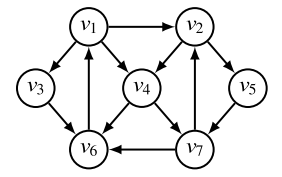
\includegraphics[width=0.4\textwidth]{Fig_1_30.png}

\textbf{Vertices}: $v_1, v_2, v_3, v_4, v_5, v_6, v_7$

\textbf{Edges in the undirected version}:
\[
\begin{aligned}
&v_1 - v_2,\quad v_1 - v_3,\quad v_1 - v_4,\quad v_2 - v_4,\quad v_2 - v_5, \quad v_1 - v_6, \\
&v_3 - v_6,\quad v_4 - v_6,\quad v_4 - v_7,\quad v_5 - v_7,\quad v_6 - v_7, \quad v_2 - v_7
\end{aligned}
\]

There are $7$ vertices and $12$ edges in the undirected version. A spanning tree of this graph will have exactly $6$ edges and no cycles.

\textbf{Solution}

Spanning tree of the graph in Fig. 1.30:
\begin{align*}
    T_1 &= \{ \{v_1 \to v_2\}, \{v_2 \to v_5\}, \{v_5 \to v_7\}, \{v_1 \to v_3\}, \{v_3 \to v_6\}, \{v_1 \to v_4\} \} \\
    T_2 &= \{ \{v_1 \to v_2\}, \{v_2 \to v_5\}, \{v_5 \to v_7\}, \{v_1 \to v_3\}, \{v_3 \to v_6\}, \{v_2 \to v_4\} \} \\
    T_3 &= \{ \{v_1 \to v_4\}, \{v_4 \to v_7\}, \{v_7 \to v_2\}, \{v_1 \to v_3\}, \{v_3 \to v_6\}, \{v_2 \to v_5\} \} \\
    T_4 &= \{ \{v_1 \to v_4\}, \{v_4 \to v_7\}, \{v_1 \to v_2\}, \{v_1 \to v_3\}, \{v_3 \to v_6\}, \{v_2 \to v_5\} \} \\
    T_5 &= \{ \{v_1 \to v_3\}, \{v_6 \to v_1\}, \{v_1 \to v_4\}, \{v_4 \to v_7\}, \{v_7 \to v_2\}, \{v_2 \to v_5\} \} \\
    T_6 &= \{ \{v_1 \to v_3\}, \{v_6 \to v_1\}, \{v_1 \to v_4\}, \{v_2 \to v_4\}, \{v_7 \to v_2\}, \{v_5 \to v_7\} \} \\
    T_7 &= \{ \{v_1 \to v_3\}, \{v_6 \to v_1\}, \{v_7 \to v_6\}, \{v_7 \to v_2\}, \{v_2 \to v_5\}, \{v_2 \to v_4\} \} \\
    T_8 &= \{ \{v_1 \to v_3\}, \{v_6 \to v_1\}, \{v_7 \to v_6\}, \{v_7 \to v_2\}, \{v_2 \to v_5\}, \{v_1 \to v_4\} \} \\
\end{align*}

\begin{verbatim}
    import networkx as nx
    
    G = nx.Graph()
    edges = [
        (1, 2), (1, 3), (1, 4),
        (2, 4), (2, 5), (3, 6),
        (4, 6), (4, 7), (5, 7), (6, 7)
    ]
    G.add_edges_from(edges)
    
    n_spanning_trees = nx.number_of_spanning_trees(G)
    print(n_spanning_trees)
\end{verbatim}

Using the code above, we can get the number of spanning trees of the underlying undirected graph in Fig. 1.30 is \textbf{288}.

\textbf{Explanation of \texttt{number\_of\_spanning\_trees()}}

The function \texttt{networkx.number\_of\_spanning\_trees(G)} returns the total number of distinct spanning trees of a connected undirected graph \( G \). 

Internally, it applies the \textbf{Matrix-Tree Theorem}, which states:

\begin{quote}
The number of spanning trees of a graph is equal to any cofactor (i.e., determinant of a minor) of its Laplacian matrix.
\end{quote}

Given a graph \( G \) with \( n \) vertices, the Laplacian matrix \( L \) is defined as:
\[
L = D - A
\]
where:
\begin{itemize}
    \item \( D \) is the degree matrix (a diagonal matrix where \( D_{ii} \) is the degree of vertex \( v_i \)),
    \item \( A \) is the adjacency matrix of the graph.
\end{itemize}

To compute the number of spanning trees, one row and the corresponding column are removed from \( L \), and the determinant of the resulting \((n-1) \times (n-1)\) matrix is taken.

This value is guaranteed to be an integer for any connected undirected graph.

\textbf{Problem 1.4}

\textbf{Extend the adjacency matrix graph representation by replacing those operations having an edge as argument or giving an edge or a list of edges as result, by corresponding operations having as argument or giving as result the source and target vertices of the edge or edges.}

\textbf{Explanation:}

In many graph libraries, edge-based operations are defined using edge objects or identifiers. However, when using an adjacency matrix representation, edges are naturally represented by ordered pairs of vertices \((v, w)\) such that the matrix entry \(A[v][w] = 1\). Therefore, we can extend and redefine these operations directly in terms of vertex pairs:

\begin{itemize}
    \item \texttt{G.del\_edge(e)} $\Rightarrow$ \texttt{G.del\_edge(v, w)} \\
    Deletes the edge from vertex \(v\) to vertex \(w\) by setting \(A[v][w] := 0\).

    \item \texttt{G.edges()} $\Rightarrow$ return all pairs \((v, w)\) such that \(A[v][w] = 1\) \\
    Returns the set of all edges as vertex pairs.

    \item \texttt{G.incoming(v)} $\Rightarrow$ return all \(u\) such that \(A[u][v] = 1\) \\
    Returns all vertices that have an edge going into vertex \(v\).

    \item \texttt{G.outgoing(v)} $\Rightarrow$ return all \(w\) such that \(A[v][w] = 1\) \\
    Returns all vertices that are targets of edges going out from vertex \(v\).

    \item \texttt{G.source(e)} $\Rightarrow$ extract \(v\) from edge \((v, w)\) \\
    The source of the edge is simply the first vertex of the pair.

    \item \texttt{G.target(e)} $\Rightarrow$ extract \(w\) from edge \((v, w)\) \\
    The target of the edge is the second vertex of the pair.
\end{itemize}

\textbf{Problem 1.5}

\textbf{Extend the first-child, next-sibling tree representation, in order to support the operations} \texttt{T.root()}, \texttt{T.number\_of\_children(v)}, \texttt{T.children(v)} \textbf{in} $\mathcal{O}(1)$ \textbf{time}.

\textbf{Solution:}

We augment the traditional first-child, next-sibling (FCNS) tree structure by storing additional information in each node and in the tree structure itself.

\begin{itemize}
    \item \texttt{T.root()}: Maintain a direct reference to the root node in the tree object \texttt{T}. Accessing the root is then a simple pointer dereference and takes constant time.

    \item \texttt{T.number\_of\_children(v)}: Add a field \texttt{v.num\_children} in each node \texttt{v}, which is incremented or decremented whenever a child is added or removed. This allows the number of children to be returned in constant time.

    \item \texttt{T.children(v)}: In addition to \texttt{v.first\_child} and \texttt{v.next\_sibling}, maintain a separate list or array \texttt{v.children[]} storing direct references to all of \texttt{v}'s children. This allows for immediate access to all children in $\mathcal{O}(1)$ time if the list is directly returned (not iterated over).
\end{itemize}

\textbf{Trade-off:}  
These enhancements increase the space complexity and require careful maintenance of the extra fields during updates (insertions, deletions). However, they provide significant performance improvements for child-related queries.

\textbf{Problem 1.6}

\textbf{Show how to double check that the graph-based representation of a tree is indeed a tree, in time linear in the size of the tree.}

To verify that a graph-based representation indeed corresponds to a valid tree, we perform the following checks in $O(n)$ time, where $n$ is the number of nodes in the graph:

\begin{enumerate}
    \item \textbf{Check for exactly one root node.}
    
    A root node is defined as a node with no incoming edges. We iterate through all nodes and count how many satisfy this condition:
    \[
    \text{root\_count} \gets 0
    \]
    \[
    \text{for each } v \in T.vertices(): \quad \text{if } T.incoming(v).empty(): \quad \text{root\_count} \gets \text{root\_count} + 1
    \]
    If $\text{root\_count} \ne 1$, the structure is not a valid tree.

    \item \textbf{Check that every non-root node has exactly one parent.}
    
    For each node $v$ with incoming edges, we ensure:
    \[
    \text{if } \neg T.incoming(v).empty(), \text{ then } T.incoming(v).size() = 1
    \]
    This guarantees that every node except the root has exactly one parent.

    \item \textbf{Check for connectivity and absence of cycles using DFS.}
    
    We perform a depth-first search (DFS) from the root node and:
    \begin{itemize}
        \item Mark each visited node to avoid revisiting.
        \item If a node is visited more than once, a cycle exists.
        \item If some nodes are not visited after DFS, the graph is disconnected.
    \end{itemize}

    \textit{Pseudocode:}
    \begin{verbatim}
visited = empty set

function DFS(v):
    if v in visited:
        return False  # cycle detected
    visited.add(v)
    for u in T.children(v):
        if not DFS(u):
            return False
    return True
    \end{verbatim}

    After DFS:
    \[
    \text{if } |\text{visited}| \ne T.number\_of\_nodes(), \text{ the structure is not connected.}
    \]
\end{enumerate}

\noindent
Since each operation (checking incoming/outgoing edges, DFS traversal) takes constant or linear time over all nodes and edges, the total verification process runs in $O(n)$ time.

\textbf{Exercise 1.1: The standard representation of an undirected graph in the format adopted for the DIMACS Implementation Challenges consists of a problem definition line of the form \texttt{p edge n m}, where $n$ and $m$ are, respectively, the number of vertices and the number of edges, followed by $m$ edge descriptor lines of the form \texttt{e i j}, each of them giving an edge as a pair of vertex numbers in the range $1$ to $n$. Comment lines of the form \texttt{c …} are also allowed. Implement procedures to read a DIMACS graph and to write a graph in DIMACS format.}

The DIMACS format represents an undirected graph in a standardized way:
\begin{itemize}
    \item Comment lines start with \texttt{c} and can be ignored.
    \item A line starting with \texttt{p edge n m} defines the number of vertices ($n$) and edges ($m$).
    \item Each subsequent line starting with \texttt{e i j} defines an undirected edge between vertex $i$ and vertex $j$.
\end{itemize}

To handle this format, we implement two procedures:

\textbf{Reading a DIMACS graph}
We read each line of the input file:
\begin{itemize}
    \item Skip lines starting with \texttt{c}.
    \item Parse the line \texttt{p edge n m} to get the number of vertices and edges.
    \item Parse each edge line \texttt{e u v} and store the edges as pairs $(u,v)$.
\end{itemize}

\textbf{Writing a DIMACS graph}
To output a graph in DIMACS format:
\begin{itemize}
    \item Print the line \texttt{p edge n m}, where $m$ is the number of edges.
    \item For each edge $(u, v)$, write the line \texttt{e u v}.
\end{itemize}

\textbf{Exercise 1.2: The external representation of a graph in the Stanford GraphBase (SGB) format consists essentially of a first line of the form \texttt{* GraphBase graph (utiltypes …,nV,mA)}, where $n$ and $m$ are, respectively, the number of vertices and the number of edges; a second line containing an identification string; a \texttt{* Vertices} line; $n$ vertex descriptor lines of the form \texttt{label,Ai,0,0}, where $i$ is the number of the first edge in the range $0$ to $m - 1$ going out of the vertex and \texttt{label} is a string label; an \texttt{* Arcs} line; $m$ edge descriptor lines of the form \texttt{V j,Ai,label,0}, where $j$ is the number of the target vertex in the range $0$ to $n - 1$, $i$ is the number of the next edge in the range $0$ to $m - 1$ going out of the same source vertex, and \texttt{label} is an integer label; and a last \texttt{* Checksum …} line. Further, in the description of a vertex with no outgoing edge, or an edge with no successor going out of the same source vertex, \texttt{Ai} becomes \texttt{0}. Implement procedures to read a SGB graph and to write a graph in SGB format.}

The \textbf{Stanford GraphBase (SGB)} format represents a directed graph in a structured way:

\begin{itemize}
    \item The first line begins with \texttt{* GraphBase graph (utiltypes ...,nV,mA)} where $n$ is the number of vertices and $m$ is the number of edges.
    \item The second line is an identification string (can be stored or ignored).
    \item The \texttt{* Vertices} section follows, with $n$ lines describing vertices in the format: \texttt{label,Ai,0,0}
    \begin{itemize}
        \item \texttt{label} is a string identifier.
        \item \texttt{Ai} indicates the index (from $0$ to $m-1$) of the first outgoing edge from that vertex.
        \item If there is no outgoing edge, \texttt{Ai} is \texttt{0}.
    \end{itemize}
    \item Then comes the \texttt{* Arcs} section, with $m$ lines describing directed edges (arcs) in the format: \texttt{Vj,Ai,label,0}
    \begin{itemize}
        \item \texttt{Vj} is the target vertex (in the range $0$ to $n-1$).
        \item \texttt{Ai} is the index of the next edge from the same source vertex.
        \item If there is no next edge, \texttt{Ai} is \texttt{0}.
        \item \texttt{label} is an integer label for the edge.
    \end{itemize}
    \item A final line \texttt{* Checksum ...} concludes the graph.
\end{itemize}

To process this format, we implement two procedures:

\textbf{Reading a SGB graph}
\begin{itemize}
    \item Parse the first line to extract $n$ and $m$.
    \item Skip or store the second line (identifier).
    \item In the \texttt{* Vertices} section:
    \begin{itemize}
        \item Read each vertex’s label and first outgoing edge index.
        \item Store vertex labels and associate them with outgoing edge indices.
    \end{itemize}
    \item In the \texttt{* Arcs} section:
    \begin{itemize}
        \item Read each edge’s target vertex, next edge index, and label.
        \item Construct an adjacency list or edge list accordingly.
    \end{itemize}
\end{itemize}

\textbf{Writing a SGB graph}
\begin{itemize}
    \item Output the graph header and identification string.
    \item Write the \texttt{* Vertices} section with vertex descriptors.
    \item Write the \texttt{* Arcs} section with edge descriptors.
    \item Append a \texttt{* Checksum ...} line if needed.
\end{itemize}

\begin{baitoan}[Tree edit distance]
    Viết chương trình {\sf C{\tt/}C++, Python} để giải bài toán tree edit distance problem bằng cách sử dụng: (a) Backtracking. (b) Branch-\&-bound. (c) Divide-\&-conquer -- chia để trị. (d) Dynamic programming -- Quy hoạch động.
\end{baitoan}

%------------------- Giải thích thuật toán và code tree edit distance bằng Backtracking -------------------%

\textbf{(a) Phương pháp Backtracking}

\textbf{Giải thích và công thức:}

\begin{itemize}
    \item \textbf{Bài toán:} Cho hai cây có gốc $T_1 = (V_1, E_1)$ và $T_2 = (V_2, E_2)$ (có thứ tự), tìm tất cả các ánh xạ hợp lệ từ các nút của $T_1$ sang các nút của $T_2$ (hoặc nút giả $\lambda$), tương ứng với các phép biến đổi cây (tree edit mapping).
    \item \textbf{Ý tưởng:} Duyệt tất cả các ánh xạ từng phần $M \subseteq V_1 \times (V_2 \cup \{\lambda\})$ bằng đệ quy quay lui (backtracking), đảm bảo các ràng buộc:
    \begin{itemize}
        \item Mỗi nút $v \in V_1$ được gán cho đúng một nút $w \in V_2$ cùng độ sâu (hoặc $\lambda$ nếu xóa $v$).
        \item Không có hai nút $v_1, v_2 \in V_1$ cùng gán vào một nút $w \in V_2$ (trừ $\lambda$) -- ánh xạ là song ánh trên $V_2$.
        \item Nếu $v$ là cha của $x$ trong $T_1$ và $w$ là ảnh của $v$ trong $T_2$, thì ảnh của $x$ (nếu không phải $\lambda$) phải là con của $w$ trong $T_2$.
        \item Ràng buộc thứ tự anh em: nếu $x$ là anh phải của $v$ trong $T_1$, thì ảnh của $x$ (nếu không phải $\lambda$) không được là anh trái của $w$ trong $T_2$.
    \end{itemize}
    \item \textbf{Cách xây dựng ánh xạ:}
    \begin{itemize}
        \item Duyệt các nút $v$ của $T_1$ theo thứ tự preorder.
        \item Với mỗi $v$, thử gán vào từng $w$ thuộc tập ứng viên $C[v]$ (các nút $w \in V_2$ cùng độ sâu với $v$ hoặc $\lambda$).
        \item Sau mỗi lần gán $v \to w$, cập nhật lại tập ứng viên cho các nút còn lại (loại bỏ $w$ khỏi các ứng viên khác nếu $w \neq \lambda$; loại bỏ các $y$ không phải con của $w$ khỏi ứng viên của các con $x$ của $v$; loại bỏ các $y$ vi phạm thứ tự anh em).
        \item Nếu đã gán hết các nút của $T_1$, lưu ánh xạ vào danh sách kết quả.
    \end{itemize}
    \item \textbf{Công thức đệ quy:}
    \begin{itemize}
        \item Gọi $M$ là ánh xạ hiện tại, $C$ là tập ứng viên hiện tại, $v$ là nút đang xét.
        \item Với mỗi $w \in C[v]$:
        \begin{itemize}
            \item Gán $M[v] = w$.
            \item Nếu $v$ là nút cuối cùng: lưu $M$ vào kết quả.
            \item Ngược lại: cập nhật $C$ thành $N$ bằng hàm refine (loại các ứng viên không hợp lệ), gọi đệ quy với nút tiếp theo.
        \end{itemize}
    \end{itemize}
    \item \textbf{Tập ứng viên $C[v]$:} Gồm các nút $w \in V_2$ cùng độ sâu với $v$ và nút giả $\lambda$ (tương ứng với phép xóa).
\end{itemize}

\textbf{Giải thích code:}

\begin{itemize}
    \item \textbf{Các lớp chính:}
    \begin{itemize}
        \item \texttt{TreeNode}: đại diện cho một nút của cây, gồm nhãn, danh sách con, cha, độ sâu, thứ tự preorder, thứ tự anh em.
        \item \texttt{Tree}: đại diện cho một cây, gồm danh sách nút, gốc, nút giả $\lambda$, độ sâu lớn nhất.
    \end{itemize}
    \item \textbf{Các hàm chính:}
    \begin{itemize}
        \item \texttt{assign\_preorder\_and\_depth}: Gán số preorder, độ sâu, thứ tự anh em cho từng nút bằng duyệt DFS.
        \item \texttt{add\_dummy}: Thêm nút giả $\lambda$ vào cây (dùng cho phép xóa).
        \item \texttt{set\_up\_candidate\_nodes}: Khởi tạo tập ứng viên $C[v]$ cho mỗi $v$ của $T_1$.
        \item \texttt{refine\_candidate\_nodes}: Sau khi gán $v \to w$, cập nhật lại $C$ cho các nút còn lại:
        \begin{itemize}
            \item Loại $w$ khỏi các ứng viên khác nếu $w \neq \lambda$ (ràng buộc song ánh).
            \item Với mỗi con $x$ của $v$, loại các $y$ không phải con của $w$ khỏi $C[x]$.
            \item Ràng buộc thứ tự anh em: nếu $x$ là anh phải của $v$, loại các $y$ là anh trái của $w$ khỏi $C[x]$.
        \end{itemize}
        \item \texttt{extend\_tree\_edit}: Hàm đệ quy chính, thử tất cả các ánh xạ $v \to w$ và gọi đệ quy cho nút tiếp theo.
        \item \texttt{backtracking\_tree\_edit}: Hàm tổng, khởi tạo các biến, gọi hàm đệ quy và trả về danh sách ánh xạ hợp lệ.
    \end{itemize}
    \item \textbf{Ý nghĩa các biến số chính:}
    \begin{itemize}
        \item \texttt{T1, T2}: hai cây đầu vào.
        \item \texttt{M}: ánh xạ hiện tại từ nút $T_1$ sang $T_2$ (hoặc $\lambda$).
        \item \texttt{L}: danh sách các ánh xạ hợp lệ tìm được.
        \item \texttt{C}: tập ứng viên cho từng nút $T_1$.
        \item \texttt{v, w}: nút đang xét của $T_1$ và ứng viên ánh xạ của $T_2$.
        \item \texttt{preorder\_list\_T1}: danh sách các nút $T_1$ theo thứ tự preorder.
    \end{itemize}
    \item \textbf{Độ phức tạp:} Phương pháp này liệt kê tất cả các ánh xạ hợp lệ, nên độ phức tạp là hàm mũ theo số nút.
    \item \textbf{Ưu điểm:} Đơn giản, dễ cài đặt, cho phép sinh tất cả ánh xạ hợp lệ (dùng cho kiểm thử, sinh ví dụ nhỏ).
    \item \textbf{Nhược điểm:} Không hiệu quả với cây lớn do số ánh xạ hợp lệ tăng rất nhanh.
\end{itemize}

%------------------- Hết giải thích tree edit distance bằng Backtracking -------------------%

\begin{baitoan}[Tree traversal -- Duyệt cây]
    Viết chương trình {\sf C{\tt/}C++, Python} để duyệt cây: (a) preorder traversal. (b) postorder traversal. (c) top-down traveral. (d) bottom-up traversal.
\end{baitoan}

%------------------- Giải thích thuật toán và code duyệt cây Preorder -------------------%
\textbf{(a) Preorder traversal}

\textbf{Giải thích và công thức:}

\begin{itemize}
    \item \textbf{Duyệt cây theo thứ tự trước (preorder traversal):} \textit{Preorder} là phương pháp duyệt cây mà tại mỗi nút, ta thăm nút đó trước, sau đó lần lượt duyệt các cây con từ trái sang phải.
    \item \textbf{Đệ quy:}
    \begin{itemize}
        \item Gọi $T$ là một cây gốc, $u$ là gốc của $T$, $C(u)$ là tập các con trực tiếp của $u$.
        \item Thứ tự duyệt preorder của $T$ là: đầu tiên thăm $u$, sau đó lần lượt duyệt preorder từng cây con $T_v$ với $v \in C(u)$ (theo thứ tự từ trái sang phải).
        \item Nếu $u$ là lá (không có con), chỉ thăm $u$. Nếu $u$ có các con $v_1, v_2, ..., v_k$, thì thứ tự duyệt là: $u, \text{preorder}(v_1), \text{preorder}(v_2), ..., \text{preorder}(v_k)$.
    \end{itemize}
    \item \textbf{Ý tưởng chi tiết:}
    \begin{itemize}
        \item \textbf{Bước 1:} Bắt đầu từ gốc $u$, in ra nhãn của $u$ (thăm $u$).
        \item \textbf{Bước 2:} Duyệt qua từng con $v$ của $u$ (theo thứ tự đã cho), với mỗi $v$ ta gọi đệ quy duyệt preorder cây con gốc $v$.
    \end{itemize}
\end{itemize}

\textbf{Giải thích code:}

\begin{itemize}
    \item \textbf{Biến số quan trọng:}
    \begin{itemize}
        \item $n$: số lượng đỉnh của cây.
        \item \texttt{tree}: danh sách kề, \texttt{tree[u]} chứa các con trực tiếp của đỉnh $u$.
        \item \texttt{is\_child}: mảng đánh dấu đỉnh nào là con (để tìm gốc).
        \item \texttt{root}: đỉnh gốc của cây (không là con của đỉnh nào).
    \end{itemize}
    \item \textbf{Đọc input:} Mỗi dòng gồm: $u$ $k$ $v_1$ $v_2$ ... $v_k$ (đỉnh $u$ có $k$ con là $v_1, ..., v_k$).
    \item \textbf{Hàm \texttt{preorder(u, tree)}:} In ra $u$, sau đó đệ quy duyệt từng con $v$ của $u$.
    \item \textbf{Kết quả:} In ra thứ tự các đỉnh theo duyệt preorder.
\end{itemize}

%------------------- Hết giải thích preorder -------------------%

%------------------- Giải thích thuật toán và code duyệt cây Postorder -------------------%

\textbf{(b) Postorder traversal}

\textbf{Giải thích và công thức:}

\begin{itemize}
    \item \textbf{Duyệt cây theo thứ tự sau (postorder traversal):} \textit{Postorder} là phương pháp duyệt cây mà tại mỗi nút, ta duyệt tất cả các cây con từ trái sang phải trước, sau đó mới thăm nút đó.
    \item \textbf{Đệ quy:}
    \begin{itemize}
        \item Gọi $T$ là một cây gốc, $u$ là gốc của $T$, $C(u)$ là tập các con trực tiếp của $u$.
        \item Thứ tự duyệt postorder của $T$ là: đầu tiên lần lượt duyệt postorder từng cây con $T_v$ với $v \in C(u)$ (theo thứ tự từ trái sang phải), sau đó mới thăm $u$.
        \item Nếu $u$ là lá (không có con), chỉ thăm $u$.
        \item Nếu $u$ có các con $v_1, v_2, ..., v_k$, thì thứ tự duyệt là: $\text{postorder}(v_1), \text{postorder}(v_2), ..., \text{postorder}(v_k), u$.
    \end{itemize}
    \item \textbf{Ý tưởng chi tiết:}
    \begin{itemize}
        \item \textbf{Bước 1:} Bắt đầu từ gốc $u$, lần lượt duyệt qua từng con $v$ của $u$ (theo thứ tự đã cho), với mỗi $v$ ta gọi đệ quy duyệt postorder cây con gốc $v$.
        \item \textbf{Bước 2:} Sau khi duyệt xong tất cả các con, in ra nhãn của $u$ (thăm $u$).
        \item \textbf{Bản chất:} Quá trình này là "đi hết các nhánh con trước, cha sau", đảm bảo thứ tự duyệt là: con trái $\to$ con phải $\to$ cha.
    \end{itemize}
\end{itemize}

\textbf{Giải thích code:}

\begin{itemize}
    \item \textbf{Biến số quan trọng:}
    \begin{itemize}
        \item $n$: số lượng đỉnh của cây.
        \item \texttt{tree}: danh sách kề, \texttt{tree[u]} chứa các con trực tiếp của đỉnh $u$.
        \item \texttt{is\_child}: mảng đánh dấu đỉnh nào là con (để tìm gốc).
        \item \texttt{root}: đỉnh gốc của cây (không là con của đỉnh nào).
    \end{itemize}
    \item \textbf{Đọc input:} Mỗi dòng gồm: $u$ $k$ $v_1$ $v_2$ ... $v_k$ (đỉnh $u$ có $k$ con là $v_1, ..., v_k$).
    \item \textbf{Hàm \texttt{postorder(u, tree)}:} Đầu tiên đệ quy duyệt từng con $v$ của $u$, sau đó in ra $u$.
    \item \textbf{Kết quả:} In ra thứ tự các đỉnh theo duyệt postorder.
\end{itemize}

%------------------- Hết giải thích postorder -------------------%

%------------------- Giải thích thuật toán và code duyệt cây Top-down -------------------%

\textbf{(c) Top-down traversal}

\textbf{Giải thích và công thức:}

\begin{itemize}
    \item \textbf{Duyệt cây top-down (từ gốc xuống lá):} Top-down là phương pháp duyệt cây mà tại mỗi nút, ta xử lý nút đó trước, sau đó truyền thông tin (nếu có) từ cha xuống các con, rồi tiếp tục duyệt các con. 
    \item \textbf{Thứ tự thăm:} Các đỉnh được thăm theo thứ tự không giảm của độ sâu (depth), và các đỉnh cùng độ sâu được thăm từ trái sang phải (theo thứ tự con trong danh sách kề).
    \item \textbf{Đệ quy:}
    \begin{itemize}
        \item Gọi $T$ là một cây gốc, $u$ là gốc của $T$, $C(u)$ là tập các con trực tiếp của $u$.
        \item Khi duyệt top-down, ta có thể truyền một đại lượng (ví dụ: độ sâu, tổng giá trị từ gốc đến $u$, ...) từ cha xuống con.
        \item Với mỗi lời gọi \texttt{top\_down(u, depth)}, ta xử lý $u$ ở độ sâu $depth$, sau đó lần lượt duyệt các con $v$ của $u$ với $depth+1$ (theo thứ tự trái sang phải).
        \item Ví dụ: Nếu truyền độ sâu, thì $\text{info}$ là $\text{depth}$, $\text{update}(\text{depth}) = \text{depth} + 1$.
    \end{itemize}
    \item \textbf{Ý tưởng chi tiết:}
    \begin{itemize}
        \item \textbf{Bước 1:} Bắt đầu từ gốc $u$ với thông tin ban đầu (ví dụ: depth = 0), xử lý $u$ (in ra nhãn, độ sâu, ...).
        \item \textbf{Bước 2:} Với mỗi con $v$ của $u$ (theo thứ tự trái sang phải), truyền thông tin mới (ví dụ: depth + 1) và gọi đệ quy duyệt top-down cây con gốc $v$.
        \item \textbf{Bản chất:} Tất cả các đỉnh ở độ sâu $d$ sẽ được thăm trước khi đến các đỉnh ở độ sâu $d+1$, và các đỉnh cùng độ sâu được thăm từ trái sang phải.
    \end{itemize}
\end{itemize}

\textbf{Giải thích code:}

\begin{itemize}
    \item \textbf{Biến số quan trọng:}
    \begin{itemize}
        \item $n$: số lượng đỉnh của cây.
        \item \texttt{tree}: danh sách kề, \texttt{tree[u]} chứa các con trực tiếp của đỉnh $u$.
        \item \texttt{is\_child}: mảng đánh dấu đỉnh nào là con (để tìm gốc).
        \item \texttt{root}: đỉnh gốc của cây (không là con của đỉnh nào).
        \item \texttt{depth}: độ sâu hiện tại của đỉnh $u$ (truyền từ cha xuống con).
    \end{itemize}
    \item \textbf{Đọc input:} Mỗi dòng gồm: $u$ $k$ $v_1$ $v_2$ ... $v_k$ (đỉnh $u$ có $k$ con là $v_1, ..., v_k$).
    \item \textbf{Hàm \texttt{top\_down(u, tree, depth)}:} Xử lý $u$ (in ra nhãn, độ sâu), sau đó đệ quy duyệt từng con $v$ của $u$ với $\texttt{depth}+1$ (theo thứ tự trái sang phải).
    \item \textbf{Kết quả:} In ra từng đỉnh và độ sâu tương ứng theo thứ tự top-down: các đỉnh ở độ sâu nhỏ hơn được in trước, các đỉnh cùng độ sâu in từ trái sang phải.
\end{itemize}

%------------------- Hết giải thích top-down -------------------%

%------------------- Giải thích thuật toán và code duyệt cây Bottom-up -------------------%

\textbf{(d) Bottom-up traversal}

\textbf{Giải thích và công thức:}

\begin{itemize}
    \item \textbf{Duyệt cây bottom-up (từ lá lên gốc):} Bottom-up là phương pháp duyệt cây mà các đỉnh được thăm theo thứ tự không giảm của chiều cao (height), các đỉnh cùng chiều cao được thăm theo thứ tự không giảm của độ sâu (depth), các đỉnh cùng chiều cao và độ sâu được thăm từ trái sang phải.
    \item \textbf{Thứ tự thăm:}
    \begin{itemize}
        \item Đầu tiên thăm tất cả các đỉnh có chiều cao nhỏ nhất (tức là các lá), sau đó đến các đỉnh có chiều cao lớn hơn, ... cuối cùng là gốc (chiều cao lớn nhất).
        \item Các đỉnh cùng chiều cao được thăm theo thứ tự không giảm của độ sâu (tức là các đỉnh ở gần gốc hơn được in sau).
        \item Nếu cùng chiều cao và cùng độ sâu, các đỉnh được thăm từ trái sang phải (theo thứ tự con trong danh sách kề).
    \end{itemize}
    \item \textbf{Công thức:}
    \begin{itemize}
        \item Gọi $h(u)$ là chiều cao của đỉnh $u$, $d(u)$ là độ sâu của $u$.
        \item Duyệt qua tất cả các đỉnh, sắp xếp theo bộ $(h(u), d(u), \text{thứ tự trái sang phải})$ tăng dần, rồi in ra.
        \item Chiều cao $h(u)$ được tính đệ quy: $h(u) = 1 + \max\{h(v) : v \text{ là con của } u\}$, lá có $h(u) = 0$.
    \end{itemize}
    \item \textbf{Ý tưởng chi tiết:}
    \begin{itemize}
        \item \textbf{Bước 1:} Duyệt cây để tính chiều cao và độ sâu cho từng đỉnh.
        \item \textbf{Bước 2:} Gom tất cả các đỉnh lại, sắp xếp theo chiều cao tăng dần, cùng chiều cao thì theo độ sâu tăng dần, cùng chiều cao và độ sâu thì theo thứ tự trái sang phải.
        \item \textbf{Bước 3:} In ra các đỉnh theo từng mức chiều cao.
    \end{itemize}
\end{itemize}

\textbf{Giải thích code:}

\begin{itemize}
    \item \textbf{Biến số quan trọng:}
    \begin{itemize}
        \item $n$: số lượng đỉnh của cây.
        \item \texttt{tree}: danh sách kề, \texttt{tree[u]} chứa các con trực tiếp của đỉnh $u$.
        \item \texttt{is\_child}: mảng đánh dấu đỉnh nào là con (để tìm gốc).
        \item \texttt{root}: đỉnh gốc của cây (không là con của đỉnh nào).
        \item \texttt{depths[u]}: độ sâu của đỉnh $u$.
        \item \texttt{heights[u]}: chiều cao của đỉnh $u$.
    \end{itemize}
    \item \textbf{Đọc input:} Mỗi dòng gồm: $u$ $k$ $v_1$ $v_2$ ... $v_k$ (đỉnh $u$ có $k$ con là $v_1, ..., v_k$).
    \item \textbf{Hàm \texttt{dfs\_height(u, tree, depth, depths, heights)}:} Tính đệ quy chiều cao và độ sâu cho từng đỉnh.
    \item \textbf{Hàm \texttt{bottom\_up(tree, root, n)}:} Gom thông tin các đỉnh, sắp xếp và in ra theo thứ tự bottom-up.
    \item \textbf{Kết quả:} In ra các đỉnh theo từng mức chiều cao, mỗi mức là các đỉnh cùng chiều cao, theo thứ tự độ sâu tăng dần, trái sang phải.
\end{itemize}

%------------------- Hết giải thích bottom-up -------------------%

%------------------------------------------------------------------------------%

\subsection{Breadth-first search algorithm -- Thuật toán tìm kiếm theo chiều rộng}

\begin{baitoan}
    Let $G = (V,E)$ be a finite simple graph. Implement the breadth-first search on $G$.
\end{baitoan}

%------------------- Breadth-First Search Algorithm for Simple Graph: C++ Code Explanation -------------------%

\textbf{Code Explanation:}

\begin{itemize}
    \item \textbf{Mục tiêu:} Thực hiện thuật toán duyệt theo chiều rộng (BFS) trên đồ thị đơn hữu hạn, bắt đầu từ một đỉnh cho trước.
    \item \textbf{Ý tưởng chính:} BFS duyệt đồ thị theo từng lớp, sử dụng hàng đợi (queue) để lần lượt thăm các đỉnh kề gần nhất trước.
    \item \textbf{Các biến và cấu trúc chính:}
    \begin{itemize}
        \item \texttt{adj}: Danh sách kề (adjacency list), \texttt{adj[u]} chứa các đỉnh kề với đỉnh $u$.
        \item \texttt{visited}: Mảng boolean để đánh dấu các đỉnh đã được thăm.
        \item \texttt{queue}: Hàng đợi để lưu trữ các đỉnh sẽ được thăm tiếp theo.
    \end{itemize}
    \item \textbf{Các bước chính:}
    \begin{enumerate}
        \item Nhập số đỉnh $n$, số cạnh $m$ và danh sách các cạnh.
        \item Nhập đỉnh bắt đầu $start$.
        \item Khởi tạo mảng \texttt{visited} với tất cả giá trị \texttt{false}, đánh dấu \texttt{visited[start] = true}.
        \item Đưa $start$ vào hàng đợi.
        \item Lặp cho đến khi hàng đợi rỗng:
        \begin{itemize}
            \item Lấy ra đỉnh đầu hàng đợi, in ra đỉnh đó.
            \item Với mỗi đỉnh kề chưa được thăm, đánh dấu đã thăm và đưa vào hàng đợi.
        \end{itemize}
    \end{enumerate}
    \item \textbf{Lưu ý:} Đồ thị được coi là vô hướng (undirected), nên mỗi cạnh được thêm vào cả hai chiều.
\end{itemize}

\begin{baitoan}
    Let $G = (V,E)$ be a finite multigraph. Implement the breadth-first search on $G$.
\end{baitoan}

%------------------- Breadth-First Search Algorithm for Multigraph: C++ Code Explanation -------------------%

\textbf{Code Explanation:}

\begin{itemize}
    \item \textbf{Mục tiêu:} Thực hiện thuật toán duyệt theo chiều rộng (BFS) trên đa đồ thị hữu hạn, cho phép nhiều cạnh giữa hai đỉnh nhưng không có khuyên (loop).
    \item \textbf{Ý tưởng chính:} BFS vẫn áp dụng được cho multigraph. Khi duyệt các cạnh kề, xét tất cả các cạnh (kể cả trùng lặp) giữa hai đỉnh. Đảm bảo không duyệt lại đỉnh đã thăm.
    \item \textbf{Các biến và cấu trúc chính:}
    \begin{itemize}
        \item \texttt{adj}: Danh sách kề, \texttt{adj[u]} chứa tất cả các đỉnh kề với $u$ (có thể lặp lại nếu có nhiều cạnh).
        \item \texttt{visited}: Mảng boolean để đánh dấu các đỉnh đã được thăm.
        \item \texttt{queue}: Hàng đợi để lưu trữ các đỉnh sẽ được thăm tiếp theo.
    \end{itemize}
    \item \textbf{Các bước chính:}
    \begin{enumerate}
        \item Nhập số đỉnh $n$, số cạnh $m$ và danh sách các cạnh (có thể lặp lại, không cho phép cạnh khuyên $u = v$).
        \item Nhập đỉnh bắt đầu $start$.
        \item Khởi tạo mảng \texttt{visited} với tất cả giá trị \texttt{false}, đánh dấu \texttt{visited[start] = true}.
        \item Đưa $start$ vào hàng đợi.
        \item Lặp cho đến khi hàng đợi rỗng:
        \begin{itemize}
            \item Lấy ra đỉnh đầu hàng đợi, in ra đỉnh đó.
            \item Với mỗi đỉnh kề chưa được thăm, đánh dấu đã thăm và đưa vào hàng đợi.
        \end{itemize}
    \end{enumerate}
    \item \textbf{Lưu ý:} Đa đồ thị cho phép nhiều cạnh giữa hai đỉnh, nhưng không cho phép cạnh khuyên ($u = v$). Đồ thị được coi là vô hướng (undirected), nên mỗi cạnh được thêm vào cả hai chiều.
\end{itemize}

\begin{baitoan}
    Let $G = (V,E)$ be a general graph. Implement the breadth-first search on $G$.
\end{baitoan}

%------------------- Breadth-First Search Algorithm for General Graph: C++ Code Explanation -------------------%

\textbf{Code Explanation:}

\begin{itemize}
    \item \textbf{Mục tiêu:} Thực hiện thuật toán duyệt theo chiều rộng (BFS) trên đồ thị tổng quát (general graph) hữu hạn, cho phép nhiều cạnh giữa hai đỉnh và cho phép cạnh khuyên (loop).
    \item \textbf{Ý tưởng chính:} BFS vẫn áp dụng được cho general graph. Khi duyệt các cạnh kề, xét tất cả các cạnh (kể cả trùng lặp và cạnh khuyên) giữa hai đỉnh. Đảm bảo không duyệt lại đỉnh đã thăm.
    \item \textbf{Các biến và cấu trúc chính:}
    \begin{itemize}
        \item \texttt{adj}: Danh sách kề, \texttt{adj[u]} chứa tất cả các đỉnh kề với $u$ (có thể lặp lại nếu có nhiều cạnh, và có thể có $u = v$ nếu là cạnh khuyên).
        \item \texttt{visited}: Mảng boolean để đánh dấu các đỉnh đã được thăm.
        \item \texttt{queue}: Hàng đợi để lưu trữ các đỉnh sẽ được thăm tiếp theo.
    \end{itemize}
    \item \textbf{Các bước chính:}
    \begin{enumerate}
        \item Nhập số đỉnh $n$, số cạnh $m$ và danh sách các cạnh (có thể lặp lại và có thể là cạnh khuyên).
        \item Nhập đỉnh bắt đầu $start$.
        \item Khởi tạo mảng \texttt{visited} với tất cả giá trị \texttt{false}, đánh dấu \texttt{visited[start] = true}.
        \item Đưa $start$ vào hàng đợi.
        \item Lặp cho đến khi hàng đợi rỗng:
        \begin{itemize}
            \item Lấy ra đỉnh đầu hàng đợi, in ra đỉnh đó.
            \item Với mỗi đỉnh kề chưa được thăm, đánh dấu đã thăm và đưa vào hàng đợi.
        \end{itemize}
    \end{enumerate}
    \item \textbf{Lưu ý:} Đồ thị tổng quát cho phép nhiều cạnh giữa hai đỉnh và cho phép cạnh khuyên ($u = v$). Đồ thị được coi là vô hướng (undirected), nên mỗi cạnh được thêm vào cả hai chiều (kể cả cạnh khuyên).
\end{itemize}

%------------------------------------------------------------------------------%

\subsection{Depth-first search algorithm -- Thuật toán tìm kiếm theo chiều rộng}

\begin{baitoan}
    Let $G = (V,E)$ be a finite simple graph. Implement the depth-first search on $G$.
\end{baitoan}

%------------------- Depth-First Search Algorithm for Simple Graph: C++ Code Explanation -------------------%

\textbf{Code Explanation:}

\begin{itemize}
    \item \textbf{Mục tiêu:} Thực hiện thuật toán duyệt theo chiều sâu (DFS) trên đồ thị đơn hữu hạn, bắt đầu từ một đỉnh cho trước.
    \item \textbf{Ý tưởng chính:} DFS duyệt đồ thị bằng cách đi sâu vào một nhánh trước khi quay lại và thử nhánh khác. Sử dụng đệ quy hoặc stack để thực hiện.
    \item \textbf{Các biến và cấu trúc chính:}
    \begin{itemize}
        \item \texttt{adj}: Danh sách kề (adjacency list), \texttt{adj[u]} chứa các đỉnh kề với đỉnh $u$.
        \item \texttt{visited}: Mảng boolean để đánh dấu các đỉnh đã được thăm.
        \item \texttt{stack}: Cấu trúc dữ liệu stack để lưu trữ các đỉnh cần thăm (trong phiên bản iterative).
    \end{itemize}
    \item \textbf{Các bước chính:}
    \begin{enumerate}
        \item Nhập số đỉnh $n$, số cạnh $m$ và danh sách các cạnh.
        \item Nhập đỉnh bắt đầu $start$.
        \item Khởi tạo mảng \texttt{visited} với tất cả giá trị \texttt{false}.
        \item Thực hiện DFS bằng hai cách:
        \begin{itemize}
            \item \textbf{Đệ quy:} Gọi hàm \texttt{dfs\_recursive} với đỉnh bắt đầu.
            \begin{itemize}
                \item \textbf{Cách thức:} 
                \begin{enumerate}
                    \item Đánh dấu đỉnh hiện tại là đã thăm.
                    \item In ra đỉnh hiện tại.
                    \item Với mỗi đỉnh kề chưa thăm, gọi đệ quy \texttt{dfs\_recursive(adj, visited, neighbor)}.
                    \item Khi không còn đỉnh kề nào chưa thăm, quay lại (backtrack).
                \end{enumerate}
            \end{itemize}
            \item \textbf{Iterative:} Sử dụng stack trong hàm \texttt{dfs\_iterative}.
        \end{itemize}
        \item Trong mỗi bước DFS:
        \begin{itemize}
            \item Đánh dấu đỉnh hiện tại là đã thăm.
            \item In ra đỉnh hiện tại.
            \item Thăm tất cả các đỉnh kề chưa được thăm.
        \end{itemize}
    \end{enumerate}
    \item \textbf{Lưu ý:} 
    \begin{itemize}
        \item Trong phiên bản iterative, các đỉnh kề được đẩy vào stack theo thứ tự ngược để duy trì thứ tự DFS.
        \item Đồ thị được coi là vô hướng (undirected), nên mỗi cạnh được thêm vào cả hai chiều.
    \end{itemize}
\end{itemize}

\begin{baitoan}
    Let $G = (V,E)$ be a finite multigraph. Implement the depth-first search on $G$.
\end{baitoan}

%------------------- Depth-First Search Algorithm for Multigraph: C++ Code Explanation -------------------%

\textbf{Code Explanation:}

\begin{itemize}
    \item \textbf{Mục tiêu:} Thực hiện thuật toán duyệt theo chiều sâu (DFS) trên đa đồ thị hữu hạn, cho phép nhiều cạnh giữa hai đỉnh nhưng không có khuyên (loop).
    \item \textbf{Ý tưởng chính:} DFS vẫn áp dụng được cho multigraph. Khi duyệt các cạnh kề, xét tất cả các cạnh (kể cả trùng lặp) giữa hai đỉnh. Đảm bảo không duyệt lại đỉnh đã thăm.
    \item \textbf{Các biến và cấu trúc chính:}
    \begin{itemize}
        \item \texttt{adj}: Danh sách kề, \texttt{adj[u]} chứa tất cả các đỉnh kề với $u$ (có thể lặp lại nếu có nhiều cạnh).
        \item \texttt{visited}: Mảng boolean để đánh dấu các đỉnh đã được thăm.
        \item \texttt{stack}: Cấu trúc dữ liệu stack để lưu trữ các đỉnh cần thăm (trong phiên bản iterative).
    \end{itemize}
    \item \textbf{Các bước chính:}
    \begin{enumerate}
        \item Nhập số đỉnh $n$, số cạnh $m$ và danh sách các cạnh (có thể lặp lại, không cho phép cạnh khuyên $u = v$).
        \item Nhập đỉnh bắt đầu $start$.
        \item Khởi tạo mảng \texttt{visited} với tất cả giá trị \texttt{false}.
        \item Thực hiện DFS bằng hai cách:
        \begin{itemize}
            \item \textbf{Đệ quy:} Gọi hàm \texttt{dfs\_recursive} với đỉnh bắt đầu.
            \begin{itemize}
                \item \textbf{Cách thức:} 
                \begin{enumerate}
                    \item Đánh dấu đỉnh hiện tại là đã thăm.
                    \item In ra đỉnh hiện tại.
                    \item Với mỗi đỉnh kề chưa thăm, gọi đệ quy \texttt{dfs\_recursive(adj, visited, neighbor)}.
                    \item Khi không còn đỉnh kề nào chưa thăm, quay lại (backtrack).
                \end{enumerate}
            \end{itemize}
            \item \textbf{Iterative:} Sử dụng stack trong hàm \texttt{dfs\_iterative}.
        \end{itemize}
        \item Trong mỗi bước DFS:
        \begin{itemize}
            \item Đánh dấu đỉnh hiện tại là đã thăm.
            \item In ra đỉnh hiện tại.
            \item Thăm tất cả các đỉnh kề chưa được thăm.
        \end{itemize}
    \end{enumerate}
    \item \textbf{Lưu ý:} 
    \begin{itemize}
        \item Đa đồ thị cho phép nhiều cạnh giữa hai đỉnh, nhưng không cho phép cạnh khuyên ($u = v$).
        \item Trong phiên bản iterative, các đỉnh kề được đẩy vào stack theo thứ tự ngược để duy trì thứ tự DFS.
        \item Đồ thị được coi là vô hướng (undirected), nên mỗi cạnh được thêm vào cả hai chiều.
    \end{itemize}
\end{itemize}

\begin{baitoan}
    Let $G = (V,E)$ be a general graph. Implement the depth-first search on $G$.
\end{baitoan}

%------------------- Depth-First Search Algorithm for General Graph: C++ Code Explanation -------------------%

\textbf{Code Explanation:}

\begin{itemize}
    \item \textbf{Mục tiêu:} Thực hiện thuật toán duyệt theo chiều sâu (DFS) trên đồ thị tổng quát (general graph) hữu hạn, cho phép nhiều cạnh giữa hai đỉnh và cho phép cạnh khuyên (loop).
    \item \textbf{Ý tưởng chính:} DFS vẫn áp dụng được cho general graph. Khi duyệt các cạnh kề, xét tất cả các cạnh (kể cả trùng lặp và cạnh khuyên) giữa hai đỉnh. Đảm bảo không duyệt lại đỉnh đã thăm.
    \item \textbf{Các biến và cấu trúc chính:}
    \begin{itemize}
        \item \texttt{adj}: Danh sách kề, \texttt{adj[u]} chứa tất cả các đỉnh kề với $u$ (có thể lặp lại nếu có nhiều cạnh, và có thể có $u = v$ nếu là cạnh khuyên).
        \item \texttt{visited}: Mảng boolean để đánh dấu các đỉnh đã được thăm.
        \item \texttt{stack}: Cấu trúc dữ liệu stack để lưu trữ các đỉnh cần thăm (trong phiên bản iterative).
    \end{itemize}
    \item \textbf{Các bước chính:}
    \begin{enumerate}
        \item Nhập số đỉnh $n$, số cạnh $m$ và danh sách các cạnh (có thể lặp lại và có thể là cạnh khuyên) cùng trọng số.
        \item Nhập đỉnh bắt đầu $start$.
        \item Khởi tạo mảng \texttt{visited} với tất cả giá trị \texttt{false}.
        \item Thực hiện DFS bằng hai cách:
        \begin{itemize}
            \item \textbf{Đệ quy:} Gọi hàm \texttt{dfs\_recursive} với đỉnh bắt đầu.
            \begin{itemize}
                \item \textbf{Cách thức:} 
                \begin{enumerate}
                    \item Đánh dấu đỉnh hiện tại là đã thăm.
                    \item In ra đỉnh hiện tại.
                    \item Với mỗi đỉnh kề chưa thăm, gọi đệ quy \texttt{dfs\_recursive(adj, visited, neighbor)}.
                    \item Khi không còn đỉnh kề nào chưa thăm, quay lại (backtrack).
                \end{enumerate}
            \end{itemize}
            \item \textbf{Iterative:} Sử dụng stack trong hàm \texttt{dfs\_iterative}.
        \end{itemize}
        \item Trong mỗi bước DFS:
        \begin{itemize}
            \item Đánh dấu đỉnh hiện tại là đã thăm.
            \item In ra đỉnh hiện tại.
            \item Thăm tất cả các đỉnh kề chưa được thăm.
        \end{itemize}
    \end{enumerate}
    \item \textbf{Lưu ý:} 
    \begin{itemize}
        \item Đồ thị tổng quát cho phép nhiều cạnh giữa hai đỉnh và cho phép cạnh khuyên ($u = v$).
        \item Trong phiên bản iterative, các đỉnh kề được đẩy vào stack theo thứ tự ngược để duy trì thứ tự DFS.
        \item Đồ thị được coi là vô hướng (undirected), nên mỗi cạnh được thêm vào cả hai chiều (kể cả cạnh khuyên).
    \end{itemize}
\end{itemize}

%------------------------------------------------------------------------------%

\section{Project 5: Shortest Path Problems on Graphs -- Đồ Án 5: Các Bài Toán Tìm Đường Đi Ngắn Nhất Trên Đồ Thị}

%------------------------------------------------------------------------------%

\subsection{Dijkstra's algorithm -- Thuật toán Dijkstra}

\begin{baitoan}
    Let $G = (V,E)$ be a finite simple graph. Implement the Dijkstra's algorithm to find the shortest path problem on $G$.
\end{baitoan}

%------------------- Dijkstra's Algorithm C++ Code Explanation -------------------%

% Explanation of the C++ implementation for Dijkstra's algorithm

\textbf{Code Explanation:}

\begin{itemize}
    \item \textbf{Mục tiêu:} Tìm đường đi ngắn nhất từ một đỉnh nguồn đến tất cả các đỉnh còn lại trên đồ thị đơn hữu hạn với trọng số không âm.
    \item \textbf{Ý tưởng chính:} Sử dụng hàng đợi ưu tiên (priority queue) để luôn chọn đỉnh có khoảng cách tạm thời nhỏ nhất, cập nhật dần dần các khoảng cách ngắn nhất từ nguồn đến các đỉnh.
    \item \textbf{Các biến và cấu trúc chính:}
    \begin{itemize}
        \item \texttt{adj}: Danh sách kề (adjacency list), \texttt{adj[u]} chứa các cặp $(v, w)$ với $v$ là đỉnh kề $u$, $w$ là trọng số cạnh $u-v$.
        \item \texttt{dist}: Mảng lưu khoảng cách ngắn nhất từ nguồn đến mỗi đỉnh, khởi tạo là \texttt{INF} (vô cùng lớn).
        \item \texttt{priority\_queue}: Hàng đợi ưu tiên kiểu min-heap, luôn lấy ra đỉnh có khoảng cách tạm thời nhỏ nhất.
    \end{itemize}
    \item \textbf{Các bước chính:}
    \begin{enumerate}
        \item Nhập số đỉnh $n$, số cạnh $m$ và danh sách các cạnh cùng trọng số.
        \item Nhập đỉnh nguồn $src$.
        \item Khởi tạo \texttt{dist[src] = 0}, các đỉnh còn lại là \texttt{INF}.
        \item Đưa $(0, src)$ vào hàng đợi ưu tiên.
        \item Lặp cho đến khi hàng đợi rỗng:
        \begin{itemize}
            \item Lấy ra đỉnh $u$ có khoảng cách tạm thời nhỏ nhất.
            \item Nếu đã có đường đi ngắn hơn đến $u$, bỏ qua.
            \item Với mỗi đỉnh kề $v$ của $u$, nếu tìm được đường đi ngắn hơn qua $u$, cập nhật \texttt{dist[v]} và đưa vào hàng đợi.
        \end{itemize}
        \item In ra khoảng cách ngắn nhất từ nguồn đến các đỉnh còn lại (nếu không tới được thì in \texttt{INF}).
    \end{enumerate}
\end{itemize}

%------------------------------------------------------------------------------%
\begin{baitoan}
    Let $G = (V,E)$ be a finite multigraph. Implement the Dijkstra's algorithm to find the shortest path problem on $G$.
\end{baitoan}

%------------------- Dijkstra's Algorithm for Multigraph: C++ Code Explanation -------------------%

\textbf{Code Explanation:}

\begin{itemize}
    \item \textbf{Mục tiêu:} Tìm đường đi ngắn nhất từ một đỉnh nguồn đến tất cả các đỉnh còn lại trên đồ thị đa đồ thị (multigraph) hữu hạn với trọng số không âm, cho phép nhiều cạnh giữa hai đỉnh nhưng không có khuyên (loop).
    \item \textbf{Ý tưởng chính:} Thuật toán Dijkstra vẫn áp dụng được cho multigraph. Khi duyệt các cạnh kề, xét tất cả các cạnh (kể cả trùng lặp) giữa hai đỉnh.
    \item \textbf{Các biến và cấu trúc chính:}
    \begin{itemize}
        \item \texttt{adj}: Danh sách kề, \texttt{adj[u]} chứa tất cả các cặp $(v, w)$ với $v$ là đỉnh kề $u$, $w$ là trọng số cạnh $u-v$ (có thể có nhiều cặp giống nhau nếu có nhiều cạnh).
        \item \texttt{dist}: Mảng lưu khoảng cách ngắn nhất từ nguồn đến mỗi đỉnh, khởi tạo là \texttt{INF}.
        \item \texttt{priority\_queue}: Hàng đợi ưu tiên kiểu min-heap.
    \end{itemize}
    \item \textbf{Các bước chính:}
    \begin{enumerate}
        \item Nhập số đỉnh $n$, số cạnh $m$ và danh sách các cạnh (có thể lặp lại) cùng trọng số. Nếu nhập cạnh khuyên ($u = v$), bỏ qua.
        \item Nhập đỉnh nguồn $src$.
        \item Khởi tạo \texttt{dist[src] = 0}, các đỉnh còn lại là \texttt{INF}.
        \item Đưa $(0, src)$ vào hàng đợi ưu tiên.
        \item Lặp cho đến khi hàng đợi rỗng:
        \begin{itemize}
            \item Lấy ra đỉnh $u$ có khoảng cách tạm thời nhỏ nhất.
            \item Nếu đã có đường đi ngắn hơn đến $u$, bỏ qua.
            \item Với mỗi cạnh kề $u-v$ (kể cả trùng lặp), nếu tìm được đường đi ngắn hơn qua $u$, cập nhật \texttt{dist[v]} và đưa vào hàng đợi.
        \end{itemize}
        \item In ra khoảng cách ngắn nhất từ nguồn đến các đỉnh còn lại (nếu không tới được thì in \texttt{INF}).
    \end{enumerate}
    \item \textbf{Lưu ý:} Đa đồ thị cho phép nhiều cạnh giữa hai đỉnh, nhưng không cho phép cạnh khuyên ($u = v$).
\end{itemize}

%------------------------------------------------------------------------------%
\begin{baitoan}
    Let $G = (V,E)$ be a general graph. Implement the Dijkstra's algorithm to find the shortest path problem on $G$.
\end{baitoan}

%------------------- Dijkstra's Algorithm for General Graph: C++ Code Explanation -------------------%

\textbf{Code Explanation:}

\begin{itemize}
    \item \textbf{Mục tiêu:} Tìm đường đi ngắn nhất từ một đỉnh nguồn đến tất cả các đỉnh còn lại trên đồ thị tổng quát (general graph) hữu hạn với trọng số không âm, cho phép nhiều cạnh giữa hai đỉnh và cho phép cạnh khuyên (loop).
    \item \textbf{Ý tưởng chính:} Thuật toán Dijkstra vẫn áp dụng được cho general graph. Khi duyệt các cạnh kề, xét tất cả các cạnh (kể cả trùng lặp và cạnh khuyên) giữa hai đỉnh.
    \item \textbf{Các biến và cấu trúc chính:}
    \begin{itemize}
        \item \texttt{adj}: Danh sách kề, \texttt{adj[u]} chứa tất cả các cặp $(v, w)$ với $v$ là đỉnh kề $u$, $w$ là trọng số cạnh $u-v$ (có thể có nhiều cặp giống nhau nếu có nhiều cạnh, và có thể có $u = v$ nếu là cạnh khuyên).
        \item \texttt{dist}: Mảng lưu khoảng cách ngắn nhất từ nguồn đến mỗi đỉnh, khởi tạo là \texttt{INF}.
        \item \texttt{priority\_queue}: Hàng đợi ưu tiên kiểu min-heap.
    \end{itemize}
    \item \textbf{Các bước chính:}
    \begin{enumerate}
        \item Nhập số đỉnh $n$, số cạnh $m$ và danh sách các cạnh (có thể lặp lại và có thể là cạnh khuyên) cùng trọng số.
        \item Nhập đỉnh nguồn $src$.
        \item Khởi tạo \texttt{dist[src] = 0}, các đỉnh còn lại là \texttt{INF}.
        \item Đưa $(0, src)$ vào hàng đợi ưu tiên.
        \item Lặp cho đến khi hàng đợi rỗng:
        \begin{itemize}
            \item Lấy ra đỉnh $u$ có khoảng cách tạm thời nhỏ nhất.
            \item Nếu đã có đường đi ngắn hơn đến $u$, bỏ qua.
            \item Với mỗi cạnh kề $u-v$ (kể cả trùng lặp và cạnh khuyên), nếu tìm được đường đi ngắn hơn qua $u$, cập nhật \texttt{dist[v]} và đưa vào hàng đợi.
        \end{itemize}
        \item In ra khoảng cách ngắn nhất từ nguồn đến các đỉnh còn lại (nếu không tới được thì in \texttt{INF}).
    \end{enumerate}
    \item \textbf{Lưu ý:} Đồ thị tổng quát cho phép nhiều cạnh giữa hai đỉnh và cho phép cạnh khuyên ($u = v$).
\end{itemize}

%------------------------------------------------------------------------------%
\end{document}